%*****************************************
\chapter{Results}\label{ch:results}
%*****************************************
This work describes the design and implementation of a reproducible, low-cost \ac{qa} system using two different methods for knowledge processing and answer generation - \textbf{Retrieval Augmented Generation} and \textbf{Large Context Windows}.

Different \acp{lm} provide large-context capabilities and were subsequently used within both \ac{qa} pipelines.
These models are compared with each other according to the results produced by both pipeline configurations.

\subsection*{Key Findings}\label{res:key_findings}

   Before presenting the detailed analysis of the individual evaluation criteria, the key findings of the comparison are summarised:
\begin{itemize}
    \item \textbf{Best-performing method:} 
    \begin{itemize}
        \item Overall, \textbf{\ac{rag}} has proved to be the slightly superior and more stable method.
        However, the difference compared to \ac{lcw} is model-dependent and not statistically significant.
        \item \ac{lcw} proves to be highly vulnerable to corrupted input across all evaluated models.
        \item \ac{rag} sets critical factual boundaries and maintains a high level of precision even when search queries contain spelling mistakes – This is realised at operational costs that are, in some cases, a fraction of those of the \ac{lcw} method.
    \end{itemize}
    \item \textbf{Best-performing model:}
        \begin{itemize}
            \item Across both evaluation modes, \textbf{GPT-4.1-Mini} proves to be the most balanced, accurate, and cost-effective proprietary model under \ac{rag}.
            \item The open-source model \textbf{Qwen3-VL-32B} provided by the \textit{Blablador} platform demonstrates comparatively outstanding performance, particularly in the \ac{lcw} pipeline.
            It thereby establishes itself as a high-performance, free-to-use alternative.
        \end{itemize}
    \end{itemize}

\section{Language Model Selection for Comparison}\label{sec:results_model_selection}

Selecting the appropriate \acp{lm} for a domain-specific \ac{qa} task within a cost-restricted framework requires careful balancing.
A proper weighting of resource consumption against processing capabilities is crucial.
The language models selected for the comparison are listed in \cref{tab:total_par_llm}.
%
\subsection{Final Model Selection}\label{subsec:reasoning_model}

The final decision, outlined in \cref{tab:total_par_llm_results}, has been made based on the criteria defined in \cref{subsec:model_criteria_api} and the data presented in \cref{sub:model_select_crit}.
It focuses on models that strike a balance between near-frontier execution benchmarks and minimal financial expenditure.
The benchmark results shown in \cref{tab:one_shot_llm,tab:total_par_llm,tab:qa_lcw_1_llm} indicate that the selected \acp{lm} possess significant capabilities relevant to the \ac{qa} task.

\begin{table}[H]
    \centering
    \begin{threeparttable}
    \setlength{\tabcolsep}{5pt}
    \resizebox{\textwidth}{!}{
        \begin{tabular}{lrccccccccc}
            \toprule
                                &  Total Parameters    & Context Window   & Input / Output \\
                                &                     & \footnotesize{(Tokens)} & \footnotesize{per 1M tokens (EUR)} \\
            \midrule
            Llama-4-Scout       & $109B$ ($17B$ active)  & $10M$      & $0.10 / 0.30$ \\
            DeepSeek-V3-0324    & $671B$ (37B activated) & $128,000$  & $0.20 / 0.77$  \\
            Qwen3-32B           & $32.8B$                & $131,072$  & free  \\
            Ministral-8B        & $8B$                   & $128,000$  & free \\
            Gemini-2.5-Flash    & $400B$                 & $1M$       & $0.30 / 2.50$\\
            GPT-4.1-Mini        & $\approx 7B$           & $1M$       & $0.40 / 1.60$   \\
            
            \bottomrule
        \end{tabular}}
    \caption[Total Parameters $-$ Context Window]{
        Total Parameters and Context Windows of selected models.
    }\label{tab:total_par_llm_results}
    \end{threeparttable}
\end{table}
%
\textbf{GPT-4.1-Mini}, an efficient representative of the proprietary \textit{GPT} family, is built upon an advanced autoregressive decoder-only transformer architecture.
It combines an extensive context window of $1M$ tokens while showing high-tier inference accuracy at low computational cost.
Despite its smaller size, it achieves near-top-tier results on the \textit{SimpleQA} and \textit{BoolQ} benchmarks, outperforming even the prior \ac{sota} model \textit{GPT-4o} across multiple evaluations \citep{OpenAI2025GPT_4_1}.
The model shows remarkable zero-shot capabilities, achieving leading scores on both the \textit{BoolQ} and \textit{PiQA} benchmarks.
\textit{GPT-4.1-Mini} outperforms even the much larger \textit{Llama-3.1-405B}.
Specifically, its leading score of $82.9$ on \textit{SimpleQA} highlights its ability to extract precise content with minimal hallucinations.
This represents a low-cost model with strong capabilities in retrieving accurate knowledge and clean textual definitions, making it ideal for the use case of this work.
%
\textbf{Gemini-2.5-Flash} supports a similarly large context window of $1M$ tokens while delivering extremely cost-effective performance.
Its underlying architecture uses advanced attention mechanisms and context-scaling techniques \citep{Google2025Gemini2_5}, thereby allowing the decoder to attend to large context inputs.
The \textit{Gemini-2.5-Flash} model achieves the highest score on the scientific reasoning benchmark \textit{GPQA-Diamond} ($82.8$), demonstrating high proficiency in scientific logic.
It even outperforms the \ac{sota} reference \textit{OpenAI o1}.
This outstanding performance in answering challenging multiple-choice domain expert questions \citep{rein2023gpqagraduatelevelgoogleproofqa} suggests strong results in the domain-specific \ac{qa} task evaluated in this work.

\textbf{DeepSeek-V3-0324} utilises the unique sparse \textit{DeepSeekMoE} decoder-only architecture with Multi-Head Latent Attention (MLA).
\textit{MLA} reduces the memory overhead of the key-value cache, thereby enabling highly efficient inference.
The model's sparse \textit{MoE} activates only $37$ billion parameters out of a total of $671$ billion per inference step.
In addition, \textit{DeepSeek-V3-0324} offers strong reasoning capabilities and high linguistic performance on benchmarks such as \textit{HellaSwag} at a very competitive price.
With an inference cost of \$0.20 per $1M$ input tokens, a context window of $128,000$ tokens, and the combination of \textit{MLA} and sparse \textit{MoE}, the model provides an optimal architectural balance for \ac{qa}.
The massive parameter scale is ideal for deep knowledge storage and processing.

\textbf{Llama-4-Scout} is a high-capacity, open-weight model featuring a massive context window of $10M$ tokens.
Its general benchmark results are slightly below the absolute top tier.
Nevertheless, the context capacity and low pricing of just \$0.10 per million input tokens make it an attractive alternative to the more expensive \textit{Llama-4-Maverick}.

The models \textbf{Qwen3-VL-32B-Instruct} and \textbf{Ministral-8B-Instruct-2410} \\ show lower aggregate benchmark scores but are free to use.
The possibility of inference without cost restraints represents an almost unique opportunity.
It offers broader academic access and implementation for academic practitioners and students.
The difference in benchmark values highlights the performance trade-off associated with smaller model parameters.
These alternatives also remain highly attractive in terms of privacy and resource autonomy.

All models are used \enquote{out of the box} through their respective \ac{api} providers.
The models \textit{Llama-4-Scout}, \textit{DeepSeek-V3}, \textit{Gemini-2.5-Flash}, and \textit{GPT-4.1-Mini} are accessed via \textit{OpenRouter}.

The \textit{Qwen3-VL-32B-Instruct} and \textit{Ministral-8B-Instruct-2410} models are accessed via the \textit{Blablador} platform.

\section{Evaluation Results}
The comparison criteria are \textit{Correctness}, \textit{Explainability}, \textit{Question Understanding}, and \textit{Robustness} as specified in \cref{sec:evaluation_methodology_approach}.
The procedure for carrying out this comparison is described in \cref{sec:evaluation_pipeline}.
This chapter presents and analysis the generated results step by step, categorised by the respective criteria.
The presentation of the results focuses on the individual metrics and method pipelines as a basis for the comparison.
%
\subsection{Evaluation Setup and Conditions}\label{subsec:eval_setup_conditions}

To ensure an objective and reproducible comparison between the \ac{rag} and \ac{lcw} pipelines, all experiments were conducted under identical conditions.
All models were presented with the same question sets and used \citetitle{bb2} as the knowledge base.

The parsed augmenting context is a combination of the predefined context from the question sets and the respective context determined by the method.
The evaluation process was performed entirely using the \textit{llm-as-a-judge} feature, with \textit{Gemini 2.5 Flash} as the judge.

The different question types used are listed in \cref{tab:eval_question_types}.

\begin{table}[H]
    \centering
    \begin{tabular}{lcl}
        \toprule
        \textbf{Question Type} & \textbf{Question Count} & \textbf{Description} \\
        \midrule
        Singular Fact     & 34                         & \enquote{single}     \\
        Multi Fact      & 38                         & \enquote{multi}      \\
        Transfer          & 23                         & \enquote{transfer}   \\
        \bottomrule
    \end{tabular}
    \caption[Question types of the evaluation dataset]{Question types contained in the evaluation dataset}\label{tab:eval_question_types}
\end{table}
%

The following corresponding designations are used to label the axes of the respective graphs.

\begin{table}[H]
    \centering
    \begin{tabularx}{\textwidth}{p{4.5cm}cl}
        \toprule
        \textbf{Question source} & \textbf{Number of questions} & \textbf{Designation} \\
        \midrule
        
\citetitle{bb2} by \citet{bb2} & 33 & \enquote{book} \\
        \midrule
        Oral examination questions from the module \enquote{Architecture of Information Systems in Healthcare} from 2021 & 22 & \enquote{A\_2021} \\
        
\midrule
        Written exam questions from the module \enquote{Information Systems in Healthcare and Research} from 2022 & 9 & \enquote{IS\_2022\_07\_18} \\
        
\midrule
        Written exam questions from the resit exam for the module \enquote{Information Systems in Healthcare and Research} from 2022 & 31 & \enquote{IS\_2022\_09\_27} \\
        \bottomrule
    \end{tabularx}
    
\caption[Question sources of the evaluation dataset]{Question sources contained in the evaluation dataset}\label{tab:eval_question_sources}
\end{table}
%
\paragraph{Exclusion of Ministral-8B-Instruct-2410}
During inference using both the \textit{Qwen3-VL-32B-Instruct} and \textit{Ministral-8B-Instruct-2410} from \textit{Blablador}, the models were frequently unresponsive and the \ac{api} responded with error messages.

Despite the adjustments made to the \ac{api} request, the model \textit{Ministral-8B-Instruct-2410} was unable to generate any responses (see \cref{par:inconsistent_blablador}).
This behaviour ultimately led to \textit{Ministral-8B-Instruct-2410} being excluded from the evaluation process.

%

\subsection{Correctness analysis}\label{sec:correctness_results}
\subsubsection{Total numbers}
The correctness evaluation process produces various results.
These results assess the quality of output of the \acp{lm} used in the two methods - \ac{rag} and \ac{lcw}.
The generated answers were categorised as follows:
\begin{itemize}
    \item \textit{\textcolor{red!80!black}{Not answered}} - Score \textbf{$0$}
    \item \textit{\textcolor{green!60!black}{Correct}} - Score \textbf{$1$}
    \item \textit{\textcolor{orange!80!black}{Incorrect}} - Score \textbf{$2$}
    \item \textit{\textcolor{cyan!80!black}{Partially Correct}} - Score \textbf{$3$}
\end{itemize}
There are two evaluation modes that determined the respective category of the generated answers: 
\begin{itemize}
    \item \textit{Strict} Mode
    \item \textit{Exam} Mode
\end{itemize}

\begin{table}[H]
    \centering
    \caption[Correctness - Answered - Total Numbers - \textit{Strict} Mode]{Total aggregated evaluation scores grouped by model and method - Mode \textit{Strict}.}
    \label{tab:total_strict_scores_answered}
    
    % OpenRouter Models
    \begin{threeparttable}
        \small 
        \setlength{\tabcolsep}{8pt}
        \begin{tabular}{llccccc}
            \toprule
            \textbf{Model} & \textbf{Method} & \textbf{Total} & \textbf{0} & \textbf{1} & \textbf{2} & \textbf{3} \\
            \midrule
            DeepSeek-V3 & LCW & 189 & 10 & \textbf{48} & \textbf{44} & 87 \\
            \rowcolor{gray!10} DeepSeek-V3 & RAG & 189 & 10 & 56 & 40 & 83 \\
            \addlinespace
            GPT-4.1-Mini & LCW & 189 & 8 & 47 & 49 & 85 \\
            \rowcolor{gray!10} GPT-4.1-Mini & RAG & 189 & 7 & \textbf{58} & 23 & \textbf{101} \\
            \addlinespace
            Gemini-2.5-Flash & LCW & 189 & 8 & 37 & 45 & \textbf{99} \\
            \rowcolor{gray!10} Gemini-2.5-Flash & RAG & 189 & 17 & 51 & 37 & 84 \\
            \addlinespace
            Llama-4-Scout & LCW & 189 & 8 & 43 & 53 & 85 \\
            \rowcolor{gray!10} Llama-4-Scout & RAG & 189 & \textbf{21} & 45 & 43 & 80 \\
            \bottomrule
        \end{tabular}
    \end{threeparttable}
    
    \vspace{1.5em}
    
    %Qwen Model
    \begin{threeparttable}
        \small
        \setlength{\tabcolsep}{8pt}
        \begin{tabular}{lllccccc}
            \toprule
            \textbf{Model} & \textbf{Method} & \textbf{Limit} & \textbf{Total} & \textbf{0} & \textbf{1} & \textbf{2} & \textbf{3} \\
            \midrule
            Qwen3-VL-32B & LCW & yes & 189 & \textbf{0} & 45 & 52 & \textbf{92} \\
            Qwen3-VL-32B & LCW & no & 189 & 9 & 50 & 48 & 82 \\
            \rowcolor{gray!10} Qwen3-VL-32B & RAG & yes & 189 & 11 & 36 & 53 & 89 \\
            \rowcolor{gray!10} Qwen3-VL-32B & RAG & no & 189 & 8 & \textbf{59} & \textbf{61} & 61 \\
            \bottomrule
        \end{tabular}
        
        \begin{tablenotes}\footnotesize
            \item \textbf{Scores:} \textbf{0} Not Answered, \textbf{1} Correct, \textbf{2} Incorrect, \textbf{3} Partially Correct.
            \item \textit{Upper table:} Models accessed via OpenRouter (Standard token limit $512$ on server side).
            \item \textit{Lower table:} Results of the Qwen3-VL-32B model, contrasting prompt limits.
            \item \textbf{Limit}: \textit{Token} limit defined explicitly within the prompt.\\ \textbf{No Limit}: No \textit{token} limit set.
        \end{tablenotes}
    \end{threeparttable}
\end{table}

\begin{table}[H]
    \centering
    \caption[Correctness - Answered - Percentage Rates - \textit{Strict} Mode]{Total aggregated evaluation scores represented by relative percentages grouped by model and method - Mode \textit{Strict}.}
    \label{tab:total_strict_rates_answered}
    
    % OpenRouter Models Percentages
    \begin{threeparttable}
        \small 
        \setlength{\tabcolsep}{8pt}
        \begin{tabular}{llccccc}
            \toprule
            \textbf{Model} & \textbf{Method} & \textbf{Total} & \textbf{0} & \textbf{1} & \textbf{2} & \textbf{3} \\
            \midrule
            DeepSeek-V3 & LCW & 189 & 5\% & \textbf{25\%} & \textbf{23\%} & 46\% \\
            \rowcolor{gray!10} DeepSeek-V3 & RAG & 189 & 5\% & 29\% & 21\% & 44\% \\
            \addlinespace
            GPT-4.1-Mini & LCW & 189 & 4\% & 25\% & 26\% & 45\% \\
            \rowcolor{gray!10} GPT-4.1-Mini & RAG & 189 & 4\% & \textbf{31\%} & 12\% & \textbf{53\%} \\
            \addlinespace
            Gemini-2.5-Flash & LCW & 189 & 4\% & 20\% & 24\% & 52\% \\
            \rowcolor{gray!10} Gemini-2.5-Flash & RAG & 189 & 9\% & 27\% & 20\% & 44\% \\
            \addlinespace
            Llama-4-Scout & LCW & 189 & 4\% & 23\% & 28\% & 45\% \\
            \rowcolor{gray!10} Llama-4-Scout & RAG & 189 & \textbf{11\%} & 24\% & 23\% & 42\% \\
            \bottomrule
        \end{tabular}
    \end{threeparttable}
    
    \vspace{1.5em}
    
    %Qwen Model Percentages
    \begin{threeparttable}
        \small
        \setlength{\tabcolsep}{6pt}
        \begin{tabular}{lllccccc}
            \toprule
            \textbf{Model} & \textbf{Method} & \textbf{Limit} & \textbf{Total} & \textbf{0} & \textbf{1} & \textbf{2} & \textbf{3} \\
            \midrule
            Qwen3-VL-32B & LCW & yes & 189 & \textbf{0\%} & 24\% & 28\% & \textbf{49\%} \\
            Qwen3-VL-32B & LCW & no & 189 & 5\% & 27\% & 25\% & 43\% \\
            \rowcolor{gray!10} Qwen3-VL-32B & RAG & yes & 189 & 6\% & 19\% & 28\% & 47\% \\
            \rowcolor{gray!10} Qwen3-VL-32B & RAG & no & 189 & 4\% & \textbf{31\%} & \textbf{32\%} & 32\% \\
            \bottomrule
        \end{tabular}
        
        \begin{tablenotes}\footnotesize
            \item \textbf{Scores:} \textbf{(0)} Not Answered, \textbf{(1)} Correct, \textbf{(2)} Incorrect, \textbf{(3)} Partially Correct.
            \item \textit{Upper table:} Models accessed via OpenRouter (Standard token limit $512$ on server side).
            \item \textit{Lower table:} Results of the Qwen3-VL-32B model, contrasting prompt limits.
            \item \textbf{Limit}: \textit{Token} limit defined explicitly within the prompt.\\ \textbf{No Limit}: No \textit{token} limit set.
        \end{tablenotes}
    \end{threeparttable}
\end{table}

\vspace{1cm}

The \cref{tab:total_strict_scores_answered,tab:total_strict_rates_answered} provide an overview of the aggregated evaluation scores of all generated answers regarding the evaluation in \textit{Strict} Mode.
This evaluation mode is less tolerant to indirect content and fact based subanswer matches.
%

In \cref{tab:total_strict_scores_answered,tab:total_strict_rates_answered}, the \ac{lcw} method exhibits very consistent properties across all models.
Throughout, \ac{lcw} generates a considerable number of \textit{partially correct} answers -- between $82$ and $99$ out of $189$.

This demonstrates that augmenting with the entire textbook, comprising $\approx 120,000$ tokens, successfully exposes the models to the relevant facts.
Nevertheless, they struggle to capture all required \enquote{golden} subanswers.

At the same time, the number of \textit{incorrect} answers remains remarkably high for \ac{lcw} (between $44$ and $53$ out of $189$ total answers).
Context leaks and the issues of precise and comprehensive retrieval when presented with the huge block of technical text -- comparable to looking for a \enquote{needle in a haystack} -- frequently lead to over-explanations or contextual ambiguities.
In the format of a subanswer, these ambiguities are flagged as strict mismatches when compared to the \textit{golden} subanswers.

The rate of \textit{not answered} results is low ($8$ to $10$ for \textit{OpenRouter} and even down to $0$ for a version of \textit{Qwen3-VL-32B} with restrictions).
As the entire knowledge base is available directly in the input, models almost never refuse to answer due to \enquote{insufficient information}.
The few \textit{not answered} results were mostly due to repetitive nonsensical answers by the models, which cannot be explained by the context.

The most significant difference between the two pipelines is \ac{rag}'s ability to improve precise fact retrieval.
For almost all models, switching from \ac{lcw} to \ac{rag} leads to an increase in the absolute number of \textit{Correct} classifications (Score $== 1$).

For example, \textit{DeepSeek-V3} improves from $48$ to $56$, \textit{GPT-4.1-Mini} rises from $47$ to $58$ and \textit{Gemini-2.5-Flash} from $37$ to $51$.
The precise retrieval of relevant sections of text prevents models from being distracted by irrelevant text.

However, \ac{rag} leads to a significant increase in decisions with the status \textit{Not answered} (Score $== 0$).
The number of unanswered queries for \textit{Gemini-2.5-Flash} has more than doubled (from $8$ under \ac{lcw} to $17$ under \ac{rag}), and for \textit{Llama-4-Scout} the increase is almost threefold (from $8$ to $21$).

This reflects the direct correlation between the database retrieval thresholds (similarity threshold of $0.85$) and the decision to withhold an answer -- if the vector \ac{db} cannot retrieve highly relevant points (\textit{chunks}), the models choose to withhold answers rather than generate hallucinated conclusions.

Analysis of the \textit{Qwen3-VL-32B} model under various constraint configurations shows how \textit{token} limits at the prompt level influence model outputs.

\noindent\textbf{Comparison of Methods:}
\begin{itemize}
    \item \textbf{RAG vs. LCW with limits}: The \ac{rag} method with a \textit{token} limit produces $36$ correct answers.
    The \ac{lcw} method with a \textit{token} limit achieves $45$ correct answers of $189$ total answers.
    This indicates that the \ac{lcw} method is more effective in generating correct answers when \textit{token} limits are enforced.
    \item \textbf{RAG vs. LCW without limits}: When no \textit{token} limits are applied, the \ac{rag} method achieves $59$ correct answers, while the \ac{lcw} method achieves $50$ correct answers.
    This suggests that the \ac{rag} method benefits more from unrestricted output, allowing for more comprehensive answers.
    \item \textbf{Impact of token limits}: Enforcing \textit{token} limits results in fewer \textit{not answered} questions and more \textit{partially correct} answers.
    Removing the limits allows for more correct answers but also increases the number of \textit{incorrect} answers.
\end{itemize}



\noindent\textbf{Comparison of Token Limits:}
\begin{itemize}
    \item \textbf{LCW Limit vs. No Limit}: Enforcing \textit{token} limits within the prompt results in slightly fewer \textit{correct} answers ($45$ vs. $50$ - without limits), but completely eliminates unanswered questions ($0$ vs. $9$).
    It also increases the number of \textit{partially correct} answers to $92$ from $82$.
    This suggests that \textit{token}-limited prompt instructions force the model to provide concise, truthful answers that consist of useful and relevant subanswers in context.
    On the other hand, it may happen that important subanswers are omitted more frequently if they do not match directly.
    However, these subanswers potentially contain some relevant knowledge but are avoided due to resourcefulness.
    \item \textbf{RAG Limit vs. No Limit}: The difference is even more pronounced within the \ac{rag} pipeline.
    Limiting the output \textit{tokens} results in only $36$ correct of $189$ total answers.
    If the limit is removed, the model seems to generated more comprehensive details, achieving $59$ \textit{correct} answers (the highest value in the table).
    However, this lack of restriction also causes the number of \textit{incorrect} answers to increase from $53$ to $61$.
    This suggests that long, unrestricted outputs are highly likely to contain both verified details from textbooks and incorrect statements.
    
\end{itemize}

To provide a visual, aggregated overview of these classification dynamics, \cref{fig:answered_score_stack_other_models_lcw,fig:answered_score_stack_other_models_rag,fig:answered_score_stack_qwen_lcw,fig:answered_score_stack_qwen_rag} illustrate the stacked distribution of all scored \textit{Correctness} categories.
These diagrams compare performance on questions containing intentional spelling errors with that on error-free questions (for both \ac{lcw} and \ac{rag}).

\begin{figure}[H]
    \centering
    \makebox[\textwidth][c]{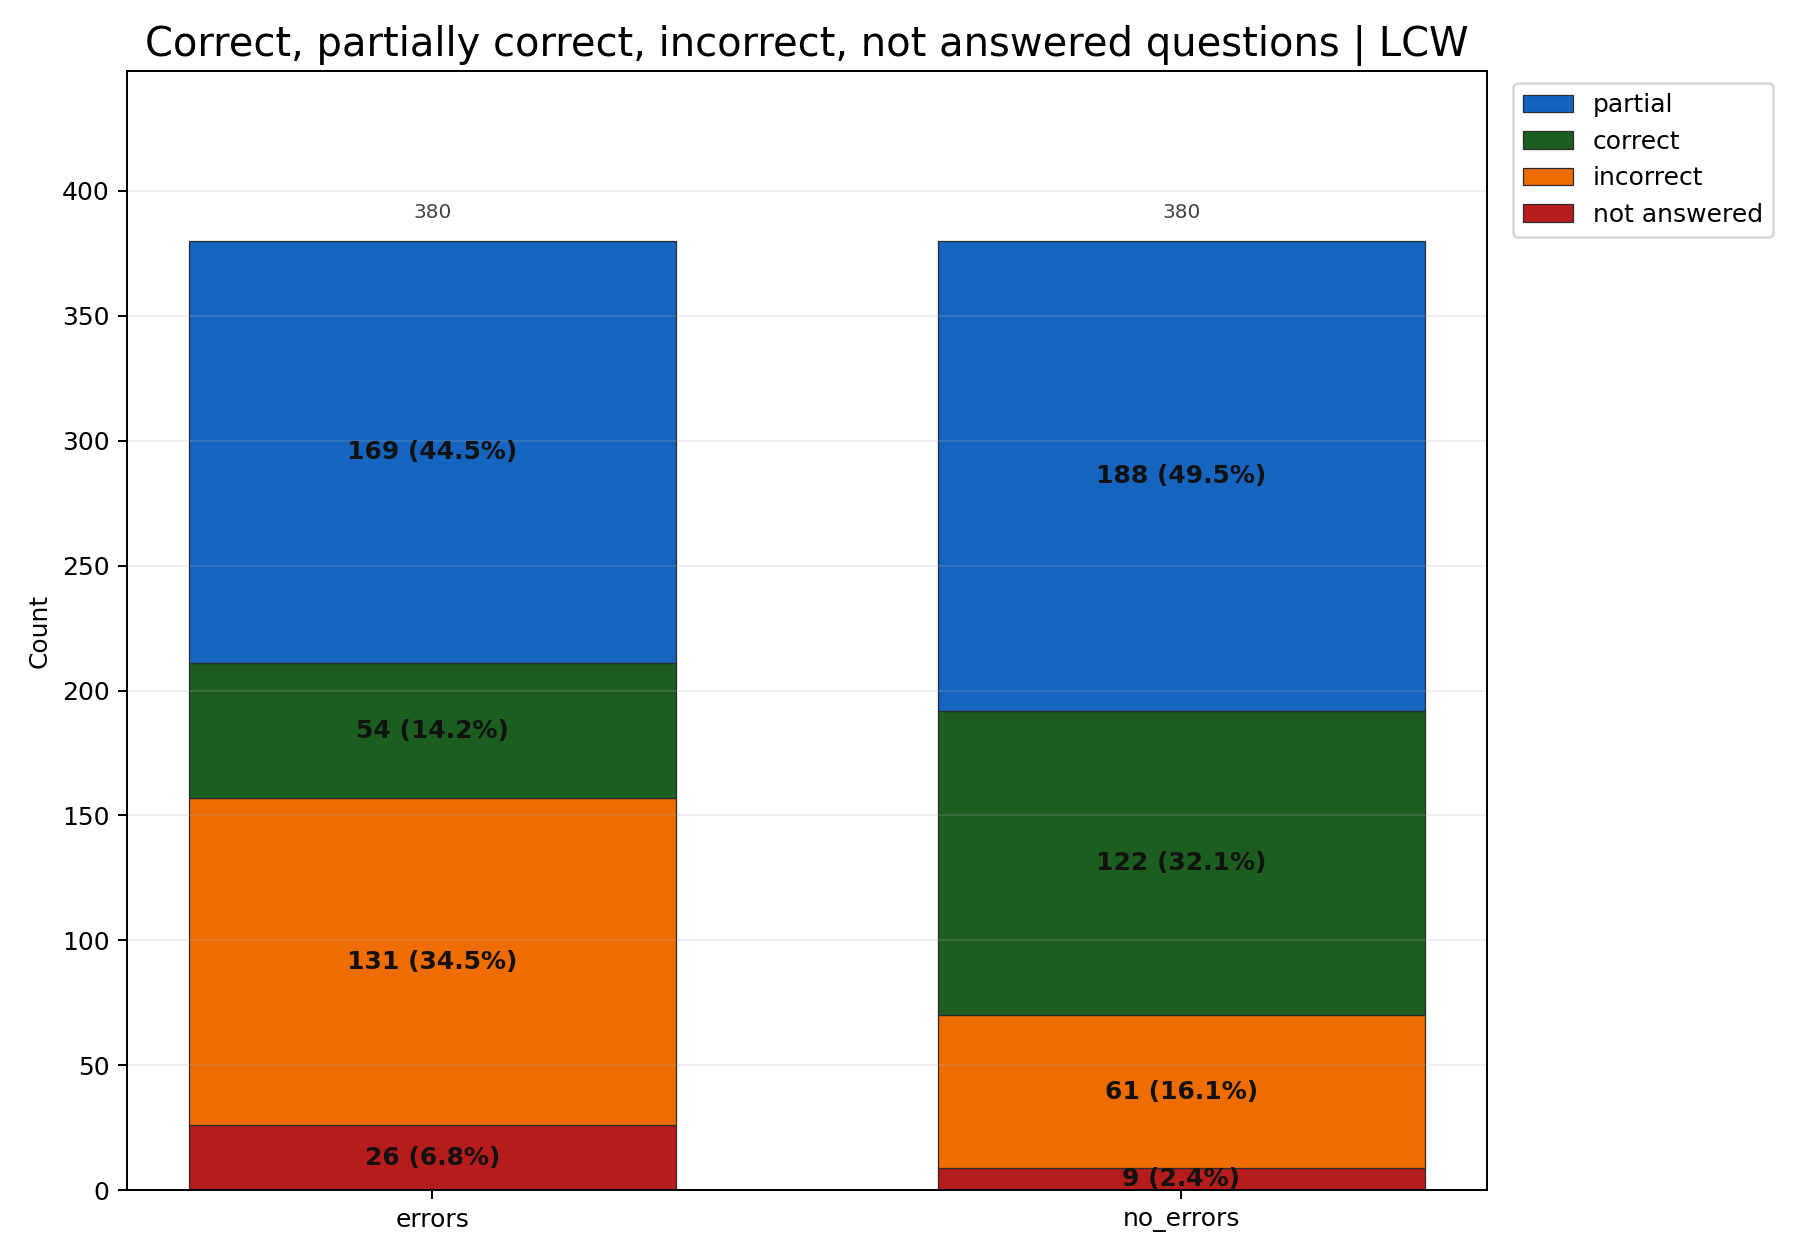
\includegraphics[width=1.12\textwidth]{figures/results/answered_score_stack_other_models_lcw_combined_limit_error.png}}
    \caption[Correctness - LCW - OpenRouter]{Correctness - Visualisation of the \textit{answered} scores for the generated results of OpenRouter models within the LCW pipeline. Comparison between questions with spelling errors (\textit{errors}) and without (\textit{no\_errors}).}\label{fig:answered_score_stack_other_models_lcw}
\end{figure}

\begin{figure}[H]
    \centering
    \makebox[\textwidth][c]{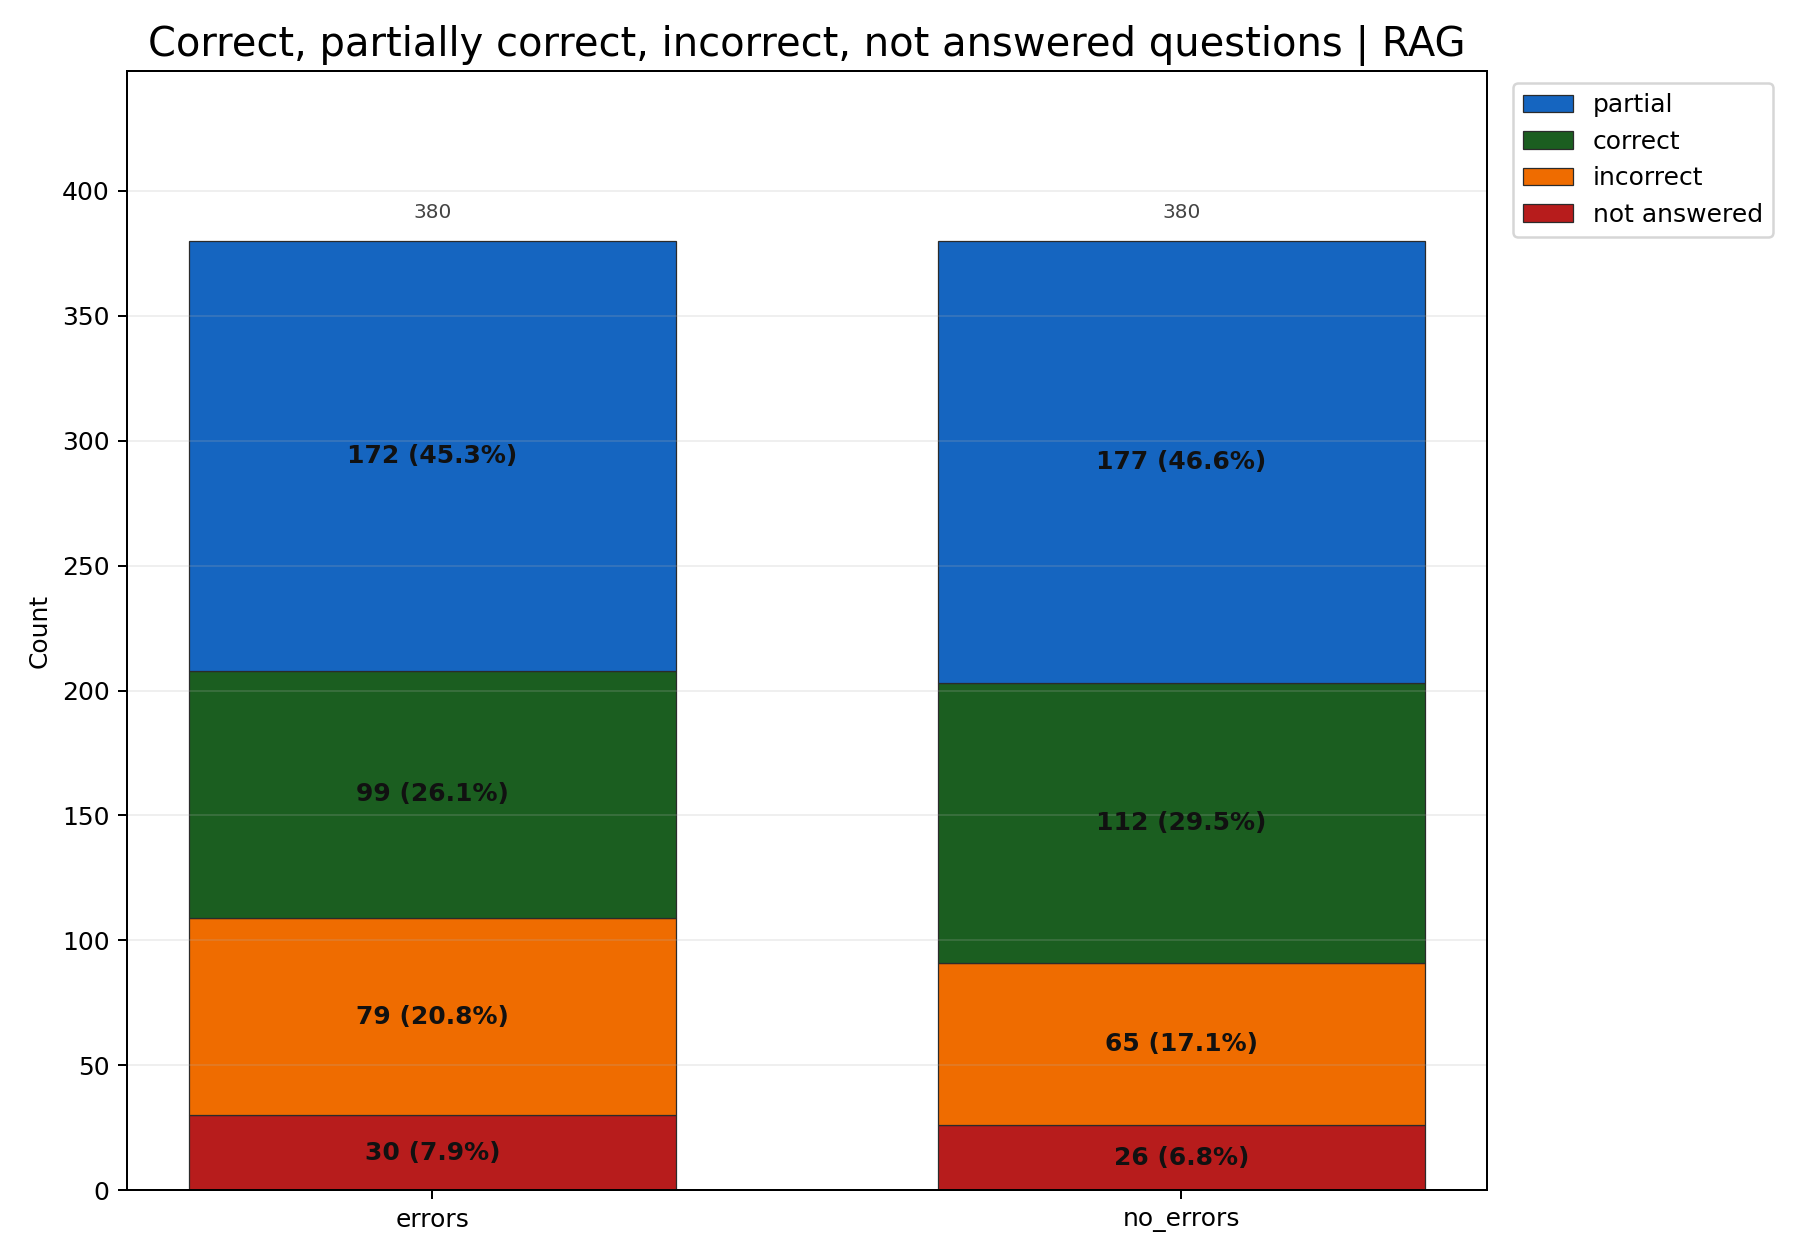
\includegraphics[width=1.12\textwidth]{figures/results/answered_score_stack_other_models_rag_combined_limit_error.png}}
    \caption[ Correctness - RAG - OpenRouter]{Correctness - Visualisation of \textit{answered} scores for the generated results of OpenRouter models within RAG pipeline.
    Comparison between questions with spelling errors (\textit{errors}) and without (\textit{no\_errors}).
    }\label{fig:answered_score_stack_other_models_rag}
\end{figure}

\begin{figure}[H]
    \centering
    \makebox[\textwidth][c]{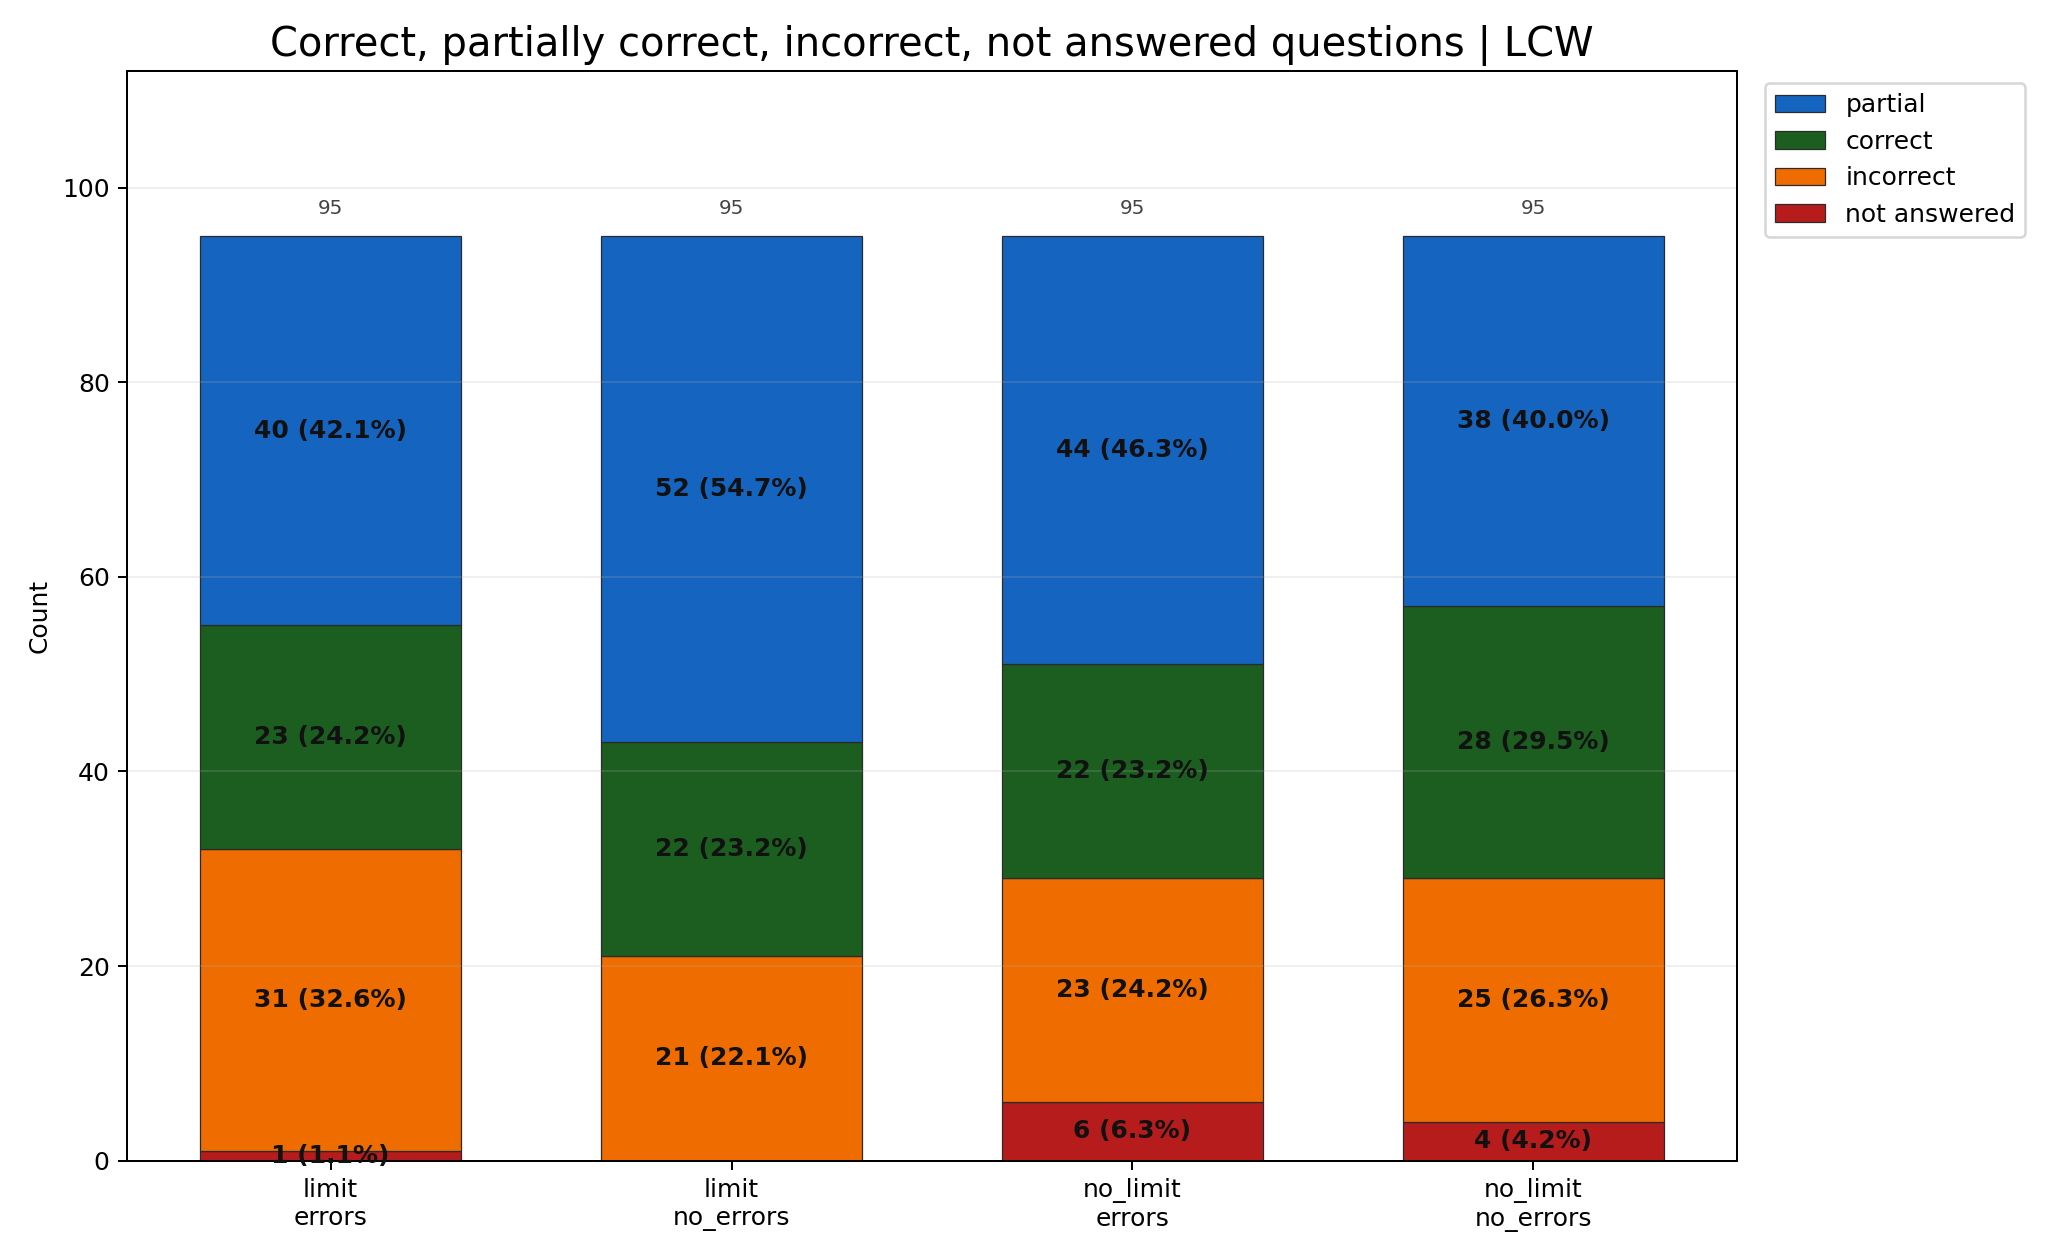
\includegraphics[width=1.12\textwidth]{figures/results/answered_score_stack_qwen_variants_lcw_combined_limit_error.png}}
    \caption[Correctness - LCW - Qwen Variants]{Correctness - Visualisation of \textit{answered} scores for the generated results of Qwen variants within LCW pipeline.
    Comparison between questions with spelling errors (\textit{errors}) and without (\textit{no\_errors}) under limit configurations.}\label{fig:answered_score_stack_qwen_lcw}
\end{figure}

\begin{figure}[H]
    \centering
    \makebox[\textwidth][c]{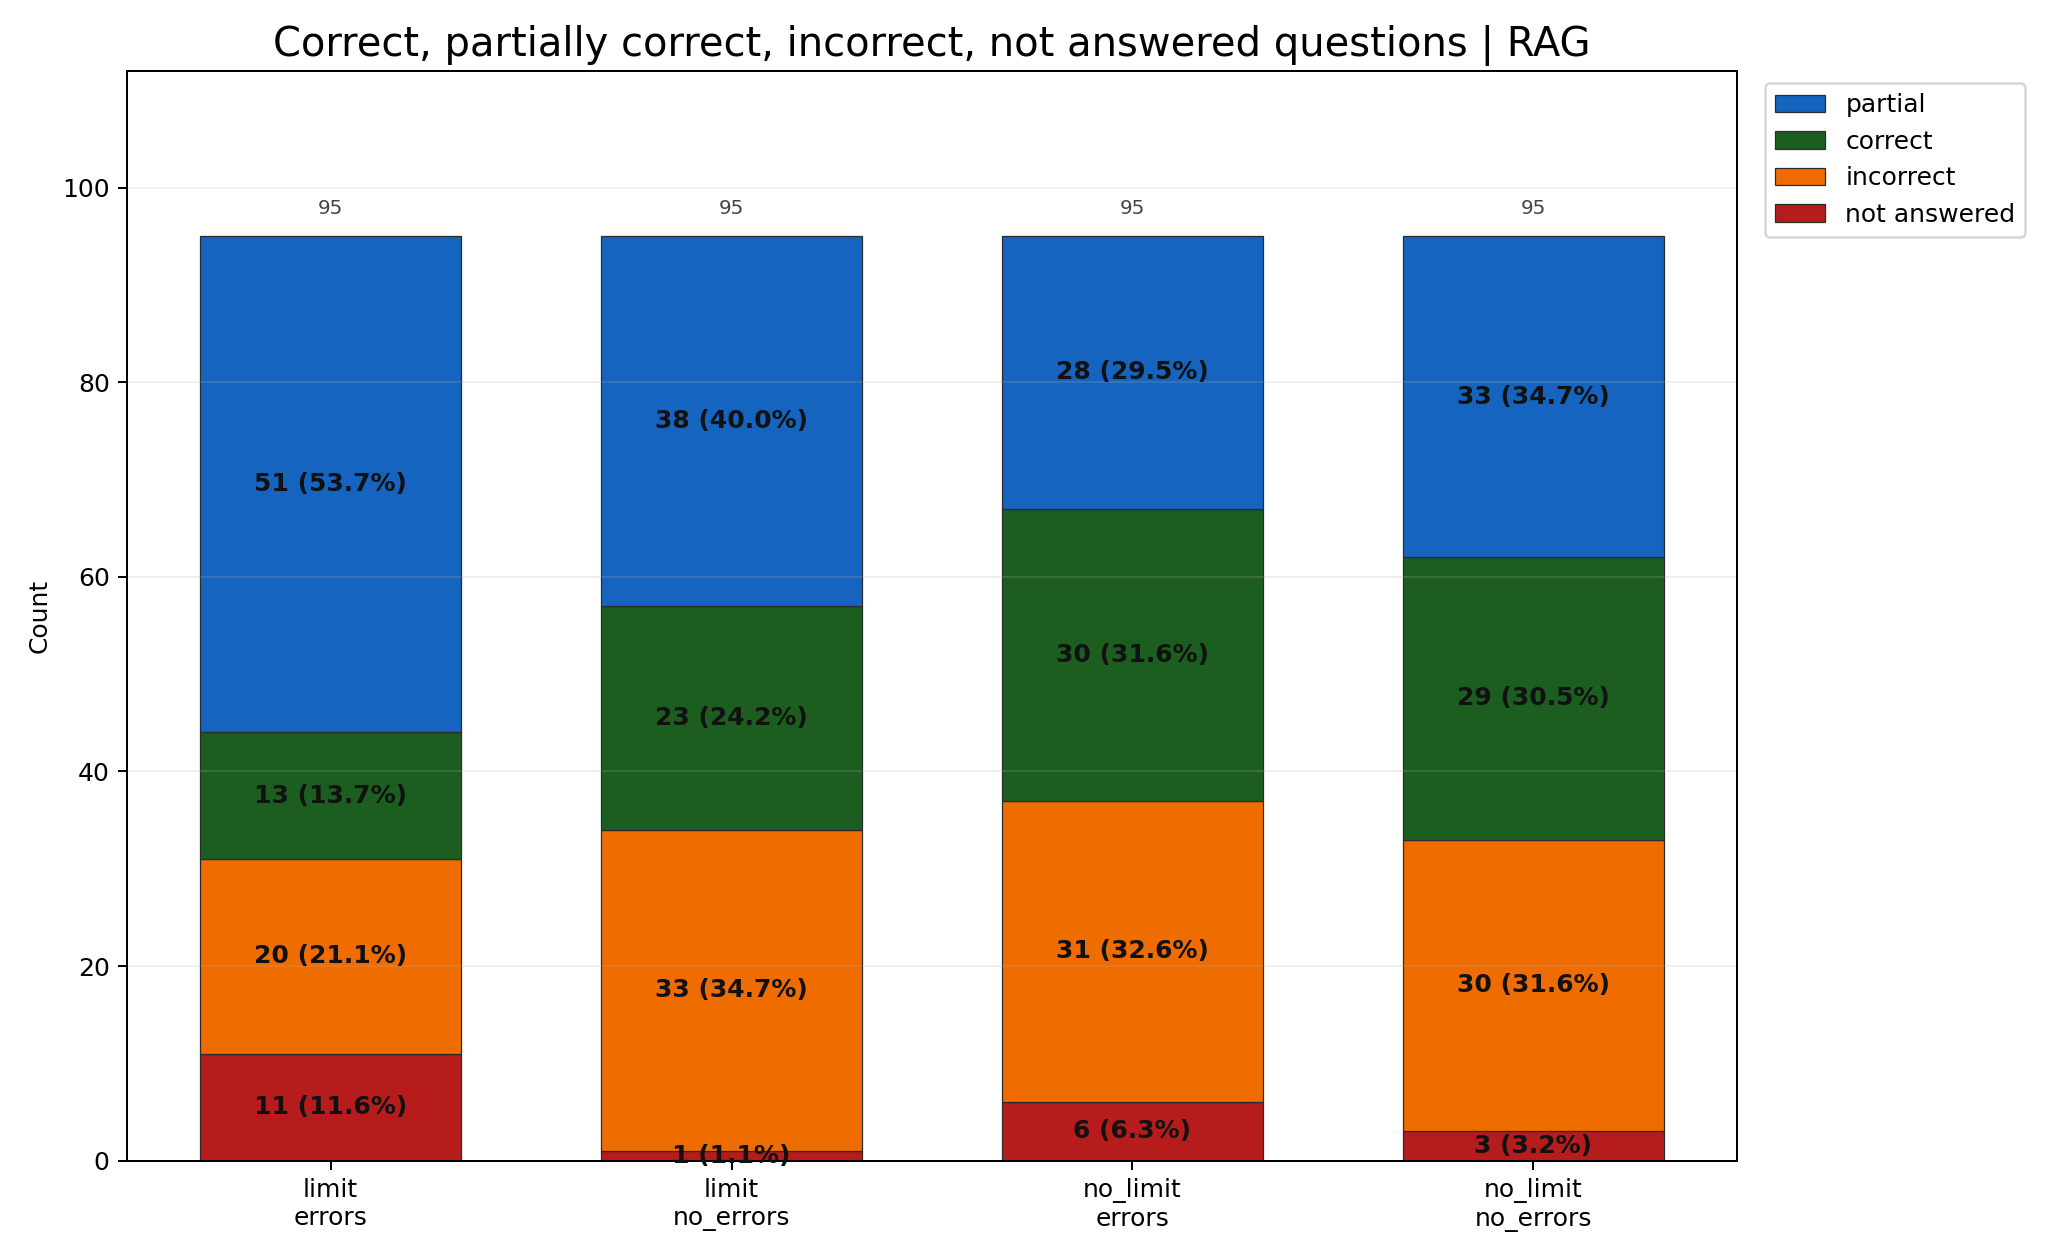
\includegraphics[width=1.12\textwidth]{figures/results/answered_score_stack_qwen_variants_rag_combined_limit_error.png}}
    \caption[Correctness - RAG - Qwen Variants]{Correctness - Visualisation of \textit{answered} scores for the generated results of Qwen variants within RAG pipeline.
    Comparison between questions with spelling errors (\textit{errors}) and without (\textit{no\_errors}) under limit configurations.}\label{fig:answered_score_stack_qwen_rag}
\end{figure}

Several macro-level insights can be derived from the distributions shown in \cref{fig:answered_score_stack_other_models_lcw,fig:answered_score_stack_other_models_rag,fig:answered_score_stack_qwen_lcw,fig:answered_score_stack_qwen_rag}:
\begin{itemize}
    \item \textbf{Loss of quality}:
    In the \ac{lcw} pipeline (\cref{fig:answered_score_stack_other_models_lcw}), questions containing spelling mistakes lead to a significant decrease in accuracy.
    The proportion of distinctly \textit{correct} answers drops from $32.1\%$ ($122$ answers) to just $14.2\%$ ($54$ answers), whilst the proportion of \textit{incorrect} answers rises from $16.1\%$ to $34.5\%$.
    This demonstrates that prompts with a long context window seem to be susceptible to noisy or corrupted inputs.
    Spelling mistakes appear to disrupt the attention mechanisms across large token ranges.
    \item \textbf{RAG Robustness}: Conversely, the \ac{rag} pipeline (\cref{fig:answered_score_stack_other_models_rag}) shows category stability despite spelling mistakes.
    Strictly \textit{correct} answers show only a slight decline from $29.5\%$ to $26.1\%$, whilst the \textit{incorrect} category rises by just $3.7$ percentage points.
    
    This stability confirms the advantage of targeted knowledge retrieval and semantic query isolation, which prevents spelling variations from affecting the context introduced during generation.

    This is also affected by expanding the original acronyms within the parsed questions for the \ac{rag} pipeline.
    Expanding the acro\-nyms was necessary to enable a targeted search in the first place (see \cref{subsec:embed_problem}).
    At the same time, the identification of relevant context became more robust, even when the input contained spelling mistakes.
    Thus, the underlying rationale introduces a positive bias that leads to an overly optimistic interpretation.
    
    
\end{itemize}
%
These figures illustrate that the similarity filter for vector queries more often prevents downstream hallucinations and instead leads models to prefer not to provide an answer rather than generate incorrect facts.

Such behaviour is preferable as it leads to higher precision.

\subsubsection{Exam Mode}\label{subsub:exam_mode_correctness}

The following table shows the numbers of the same categories assessed in \textit{Exam} mode.

% Table 2: EXAM MODE
\begin{table}[H]
    \centering
    \caption[Correctness - Answered - Total Numbers - \textit{Exam} Mode]{Total aggregated answered scores grouped by model and method - Mode \textit{Exam}.}
    \label{tab:total_exam_scores_answered}
    
    %OpenRouter Models
    \begin{threeparttable}
        \small
        \setlength{\tabcolsep}{8pt} % Reduce column padding slightly from the default 6pt/12pt
        \begin{tabular}{llccccc}
            \toprule
            \textbf{Model} & \textbf{Method} & \textbf{Total} & \textbf{0} & \textbf{1} & \textbf{2} & \textbf{3} \\
            \midrule
            DeepSeek-V3 & LCW & 189 & 10 & 53 & 25 & 101 \\
            \rowcolor{gray!10} DeepSeek-V3 & RAG & 189 & 10 & \textbf{63} & 20 & 96 \\
            \addlinespace
            GPT-4.1-Mini & LCW & 189 & 8 & 51 & 34 & 96 \\
            \rowcolor{gray!10} GPT-4.1-Mini & RAG & 189 & 7 & 61 & \textbf{13} & \textbf{108} \\
            \addlinespace
            Gemini-2.5-Flash & LCW & 189 & 8 & 43 & 31 & 107 \\
            \rowcolor{gray!10} Gemini-2.5-Flash & RAG & 189 & 17 & 56 & 30 & 86 \\
            \addlinespace
            Llama-4-Scout & LCW & 189 & 8 & 50 & 37 & 94 \\
            \rowcolor{gray!10} Llama-4-Scout & RAG & 189 & 21 & 49 & 29 & 90 \\
            \bottomrule
        \end{tabular}
    \end{threeparttable}

    \vspace{1.5em}
    
    % Qwen Model
    \begin{threeparttable}
        \small
        \setlength{\tabcolsep}{8pt}
        \begin{tabular}{lllccccc}
            \toprule
            \textbf{Model} & \textbf{Method} & \textbf{Limit} & \textbf{Total} & \textbf{0} & \textbf{1} & \textbf{2} & \textbf{3} \\
            \midrule
            Qwen3-VL-32B & LCW & yes & 189 & 0 & 57 & 24 & 108 \\
            Qwen3-VL-32B & LCW & no & 189 & 9 & 69 & 18 & 93 \\
            \rowcolor{gray!10} Qwen3-VL-32B & RAG & yes & 189 & \textbf{11} & 45 & 31 & 102 \\
            \rowcolor{gray!10} Qwen3-VL-32B & RAG & no & 189 & 8 & 68 & 27 & 86 \\
            \bottomrule
        \end{tabular}
        
        \begin{tablenotes}\footnotesize
            \item \textbf{Scores}: \textbf{0} Not Answered, \textbf{1} Correct, \textbf{2} Incorrect, \textbf{3} Partially Correct.
            \item \textit{Upper table:} Models accessed via OpenRouter (Standard \textit{token} limit $512$ on server side).
            \item \textit{Lower table:} Results of the Qwen3-VL-32B model, contrasting prompt limits.
            \item \textbf{Limit}: \textit{Token} limit defined explicitly within the prompt.\\ \textbf{No Limit}: No \textit{token} limit set.
        \end{tablenotes}
    \end{threeparttable}
\end{table}

\begin{table}[H]
    \centering
    \caption[Correctness - Answered - Percentage Rates - \textit{Exam} Mode]{Total aggregated answered scores represented by relative percentages grouped by model and method - Mode \textit{Exam}.}
    \label{tab:total_exam_rates_answered}
    
    %OpenRouter Models
    \begin{threeparttable}
        \small
        \setlength{\tabcolsep}{8pt}
        \begin{tabular}{llccccc}
            \toprule
            \textbf{Model} & \textbf{Method} & \textbf{Total} & \textbf{0} & \textbf{1} & \textbf{2} & \textbf{3} \\
            \midrule
            DeepSeek-V3 & LCW & 189 & 5\% & 28\% & 13\% & 53\% \\
            \rowcolor{gray!10} DeepSeek-V3 & RAG & 189 & 5\% & 33\% & 11\% & 51\% \\
            \addlinespace
            GPT-4.1-Mini & LCW & 189 & 4\% & 27\% & 18\% & 51\% \\
            \rowcolor{gray!10} GPT-4.1-Mini & RAG & 189 & 4\% & 32\% & 7\% & 57\% \\
            \addlinespace
            Gemini-2.5-Flash & LCW & 189 & 4\% & 23\% & 16\% & \textbf{57\%} \\
            \rowcolor{gray!10} Gemini-2.5-Flash & RAG & 189 & 9\% & 30\% & 16\% & 46\% \\
            \addlinespace
            Llama-4-Scout & LCW & 189 & 4\% & 27\% & 20\% & 50\% \\
            \rowcolor{gray!10} Llama-4-Scout & RAG & 189 & \textbf{11\%} & 26\% & 15\% & 48\% \\
            \bottomrule
        \end{tabular}
    \end{threeparttable}

    \vspace{1.5em}
    
    % Qwen Model
    \begin{threeparttable}
        \small
        \setlength{\tabcolsep}{8pt}
        \begin{tabular}{lllccccc}
            \toprule
            \textbf{Model} & \textbf{Method} & \textbf{Limit} & \textbf{Total} & \textbf{0} & \textbf{1} & \textbf{2} & \textbf{3} \\
            \midrule
            Qwen3-VL-32B & LCW & yes & 189 & 0\% & 30\% & 13\% & \textbf{57\%} \\
            Qwen3-VL-32B & LCW & no & 189 & 5\% & 37\% & \textbf{10\%} & 49\% \\
            \rowcolor{gray!10} Qwen3-VL-32B & RAG & yes & 189 & 6\% & 24\% & 16\% & 54\% \\
            \rowcolor{gray!10} Qwen3-VL-32B & RAG & no & 189 & 4\% & 36\% & 14\% & 46\% \\
            \bottomrule
        \end{tabular}
        
        \begin{tablenotes}\footnotesize
            \item \textbf{Scores}: \textbf{(0)} Not Answered, \textbf{(1)} Correct, \textbf{(2)} Incorrect, \textbf{(3)} Partially Correct.
            \item \textit{Upper table:} Models accessed via OpenRouter (Standard \textit{token} limit $512$ on server side).
            \item \textit{Lower table:} Results of the Qwen3-VL-32B model, contrasting prompt limits.
            \item \textbf{Limit}: \textit{Token} limit defined explicitly within the prompt.\\ \textbf{No Limit}: No \textit{token} limit set.
            \item Percentage values are rounded to the nearest whole number.
        \end{tablenotes}
    \end{threeparttable}
\end{table}

The generated answers in \cref{tab:total_exam_scores_answered} show slightly higher success rates within both methods than those previously assessed in \textit{Strict} mode.
The \textit{Exam} mode reassesses subanswers that were previously classified as \textit{helpful} into the \textit{correct} class.
Thereby, increasing the overall points and subsequently the count of correctly answered questions.

Similar to the results in \cref{tab:total_strict_scores_answered}, the \textit{DeepSeek V3} ($53$ - LCW, $63$ - RAG) and \textit{GPT 4.1 Mini} ($51$ - LCW, $61$ - RAG) models perform better than \textit{Llama 4 Scout} ($50$ - LCW, $49$ - RAG) and \textit{Gemini 2.5 Flash} ($43$ - LCW, $56$ - RAG) models.

The \textit{Qwen3-VL-32B} model also generates more correctly answered questions without a set \textit{token} limit than with a limit.

The total numbers indicate a generally low success rate across all models and methods.

Within the scope of this work, it has to be again emphasised that the underlying \textit{incorrect} assessment of the subanswers is based on a strict comparison with the \textit{golden} subanswers.
This frequently results in a high number of an overall \textit{incorrect} classifications of the answer, even if the model has provided a predominant amount of correct subanswers.

The results should be interpreted as a representation of the methodological framework and not of the models and methods in general.
Furthermore, this initial impression is slightly revised considering the \textit{partially correct} answers, as outlined in \cref{subsub:correct_partially_combined}.

Despite the overall low success rates, certain differences and trends can be observed.

\subsubsection{Not answered}

Only a few questions were evaluated as \textit{unanswered} (\textit{answered} score $== 0$).
By contrast, the \ac{rag} method resulted in more \textit{unanswered} questions.

Particularly for the \textit{Gemini-2.5 Flash} and \textit{Llama-4 Scout} models, the \ac{rag} method shows two to three times more unanswered questions.
The inability to answer questions within the \ac{rag} method is significantly influenced by the quantity and quality of the retrieved and parsed chunks.

If no \textit{chunks} are provided to the model as context, the models frequently indicated insufficient context and did not answer the respective questions.

This behaviour is preferred.
It avoids obtaining fictional answers or those that are not based exclusively on the knowledge base.
Otherwise, a model would rely on pre-trained knowledge, which most likely deviates from the textbook used as the knowledge base.
%
\subsubsection{Partially Correct}
Significantly high figures are shown in the \textit{Partially Correct} class.

The significance of these figures is explained in more detail in \cref{subsub:correct_partially_combined}.


\subsubsection{Correct + Partially Correct}\label{subsub:correct_partially_combined}

The results of questions directly and unequivocally classified as \textit{correct} suggest, in themselves, that the models and methods performed poorly.

However, if the \textit{partially correct} values are included in the overall assessment, this impression changes.
Unequivocally \textit{correct} refers to answers that match the golden true answers exactly.
This means that all subanswers of the golden true answer have at least one direct match with a generated subanswer.
Furthermore, no generated subanswer of the complete answer contains information that is contradicted or incorrect. 

\textit{Partially correct} answers have almost the same properties.
However, a direct match could not be found for every golden true subanswer.
This therefore constitutes an \textit{underfit}.
Nevertheless, all generated subanswers contain valuable and well-founded knowledge in relation to the question and the knowledge base.

In view of this, combining the \textit{correct} and \textit{partially correct} answers provides a more comprehensive insight into performance.

\begin{table}[htbp]
    \centering
    \caption[\textit{Answered} scores - \textit{Correct} $+$ \textit{Partially Correct}]{Sum of aggregated \textit{Correct} and \textit{Partially Correct} scores and their percentage of the total number of questions - Mode \textit{Strict}.}
    \label{tab:total_strict_combined_scores_answered}
    
    % OpenRouter Models
    \begin{threeparttable}
        \small 
        \begin{tabular}{llccccc}
            \toprule
            \textbf{Model} & \textbf{Method} & \textbf{Total} & \textbf{(1)} $+$ \textbf{(3)} & \textbf{\%} \\
            \midrule
            DeepSeek-V3 & LCW & 189 & 135 & \textbf{71} \\
            \rowcolor{gray!10} DeepSeek-V3 & RAG & 189 & 139 & \textbf{73} \\
            \addlinespace
            GPT-4.1-Mini & LCW & 189 & 132 & \textbf{69} \\
            \rowcolor{gray!10} GPT-4.1-Mini & RAG & 189 & 159 & \textbf{84} \\
            \addlinespace
            Gemini-2.5-Flash & LCW & 189 & 136 & \textbf{71} \\
            \rowcolor{gray!10} Gemini-2.5-Flash & RAG & 189 & 135 & \textbf{71} \\
            \addlinespace
            Llama-4-Scout & LCW & 189 & 128 & \textbf{67} \\
            \rowcolor{gray!10} Llama-4-Scout & RAG & 189 & 125 & \textbf{66} \\
            \bottomrule
        \end{tabular}
    \end{threeparttable}
    
    \vspace{1.5em}
    
    %Qwen Model
    \begin{threeparttable}
        \small
        \begin{tabular}{lllccccc}
            \toprule
            \textbf{Model} & \textbf{Method} & \textbf{Limit} & \textbf{Total} & \textbf{(1)} $+$ \textbf{(3)} & \textbf{\%} \\
            \midrule
            Qwen3-VL-32B & LCW & yes & 189 & 137 & \textbf{72} \\
            Qwen3-VL-32B & LCW & no & 189 & 132 & \textbf{69} \\
            \rowcolor{gray!10} Qwen3-VL-32B & RAG & yes & 189 & 125 & \textbf{66} \\
            \rowcolor{gray!10} Qwen3-VL-32B & RAG & no & 189 & 120 & \textbf{63} \\
            \bottomrule
        \end{tabular}
        
        \begin{tablenotes}\footnotesize
            \item \textbf{Scores:} \textbf{(0)} Not Answered, \textbf{(1)} Correct, \textbf{(2)} Incorrect, \textbf{(3)} Partially Correct.
            \item \textit{Upper table:} Models accessed via OpenRouter (Standard \textit{token} limit $512$ on server side).
            \item \textit{Lower table:} Results of the Qwen3-VL-32B model, contrasting prompt limits.
            \item \textbf{Limit}: \textit{token} limit defined explicitly within prompt. \textbf{No Limit}: No \textit{token} limit set.
        \end{tablenotes}
    \end{threeparttable}
\end{table}

%%%
%
%
%
%
%
%
%%%
%
%
\begin{table}[htbp]
    \centering
    \caption[\textit{Answered} Scores - \textit{Correct} $+$ \textit{Partially Correct}]{Sum of aggregated \textit{Correct} and \textit{Partially Correct} scores and their percentage of the total number of questions - Mode \textit{Exam}.}
    \label{tab:total_combined_exam_scores_answered}
    
    %OpenRouter Models
    \begin{threeparttable}
        \small
        \begin{tabular}{llccccc}
            \toprule
            \textbf{Model} & \textbf{Method} & \textbf{Total} & \textbf{(1)} $+$ \textbf{(3)} & \textbf{\%} \\
            \midrule
            DeepSeek-V3 & LCW & 189 & 154 & 81 \\
            \rowcolor{gray!10} DeepSeek-V3 & RAG & 189 & 159 & 84 \\
            \addlinespace
            GPT-4.1-Mini & LCW & 189 & 147 & 77 \\
            \rowcolor{gray!10} GPT-4.1-Mini & RAG & 189 & 169 & 89 \\
            \addlinespace
            Gemini-2.5-Flash & LCW & 189 & 150 & 79 \\
            \rowcolor{gray!10} Gemini-2.5-Flash & RAG & 189 & 142 & 75 \\
            \addlinespace
            Llama-4-Scout & LCW & 189 & 134 & 71 \\
            \rowcolor{gray!10} Llama-4-Scout & RAG & 189 & 139 & 74 \\
            \bottomrule
        \end{tabular}
    \end{threeparttable}

    \vspace{1.5em}
    
    % Qwen Model
    \begin{threeparttable}
        \small
        \begin{tabular}{lllccccc}
            \toprule
            \textbf{Model} & \textbf{Method} & \textbf{Limit} & \textbf{Total} & \textbf{(1) + (3)} & \textbf{\%} \\
            \midrule
            Qwen3-VL-32B & LCW & yes & 189 & 165 & 87\\
            Qwen3-VL-32B & LCW & no & 189 & 159 & 84 \\
            \rowcolor{gray!10} Qwen3-VL-32B & RAG & yes & 189 & 147 & 77 \\
            \rowcolor{gray!10} Qwen3-VL-32B & RAG & no & 189 & 154 & 81 \\
            \bottomrule
        \end{tabular}
        
        \begin{tablenotes}\footnotesize
            \item \textbf{Scores:} \textbf{(0)} Not Answered, \textbf{(1)} Correct, \textbf{(2)} Incorrect, \textbf{(3)} Partially Correct.
            \item \textit{Upper table:} Models accessed via OpenRouter (Standard \textit{token} limit $512$ on server side).
            \item \textit{Lower table:} Results of the Qwen3-VL-32B model, contrasting prompt limits.
            \item \textbf{Limit}: \textit{Token} limit defined explicitly within prompt. \textbf{No Limit}: No \textit{token} limit set.
        \end{tablenotes}
    \end{threeparttable}
\end{table}
%

The combined results in \cref{tab:total_combined_exam_scores_answered} and \cref{tab:total_strict_combined_scores_answered} show a significant improvement in performance.

Overall, neither of the two methods demonstrates consistently superior performance.

\textit{Partially correct} answers are also knowledge-enriching and valuable to the defined target group in terms of reliably answering the question.
%
Taking these answers into account is therefore important for evaluating the methodology.
%
\subsection{Macro F1}

The total numbers shown in \cref{tab:total_exam_scores_answered} and \cref{tab:total_strict_scores_answered} are reflected accordingly in the \textit{F1} values.

The Macro \textit{F1} score ranges from \numrange{0}{1} and provides a comprehensive representation of the actual performance of the respective model.

Models that have answered questions correctly but have also provided incorrect or incomplete answers receive a lower \textit{F1} score.
A model with a Macro \textit{F1} score of \num{0} answers no questions correctly, whilst a model with a score of \num{1} answers all questions correctly and completely.
%

\begin{figure}[H]
    \centering
    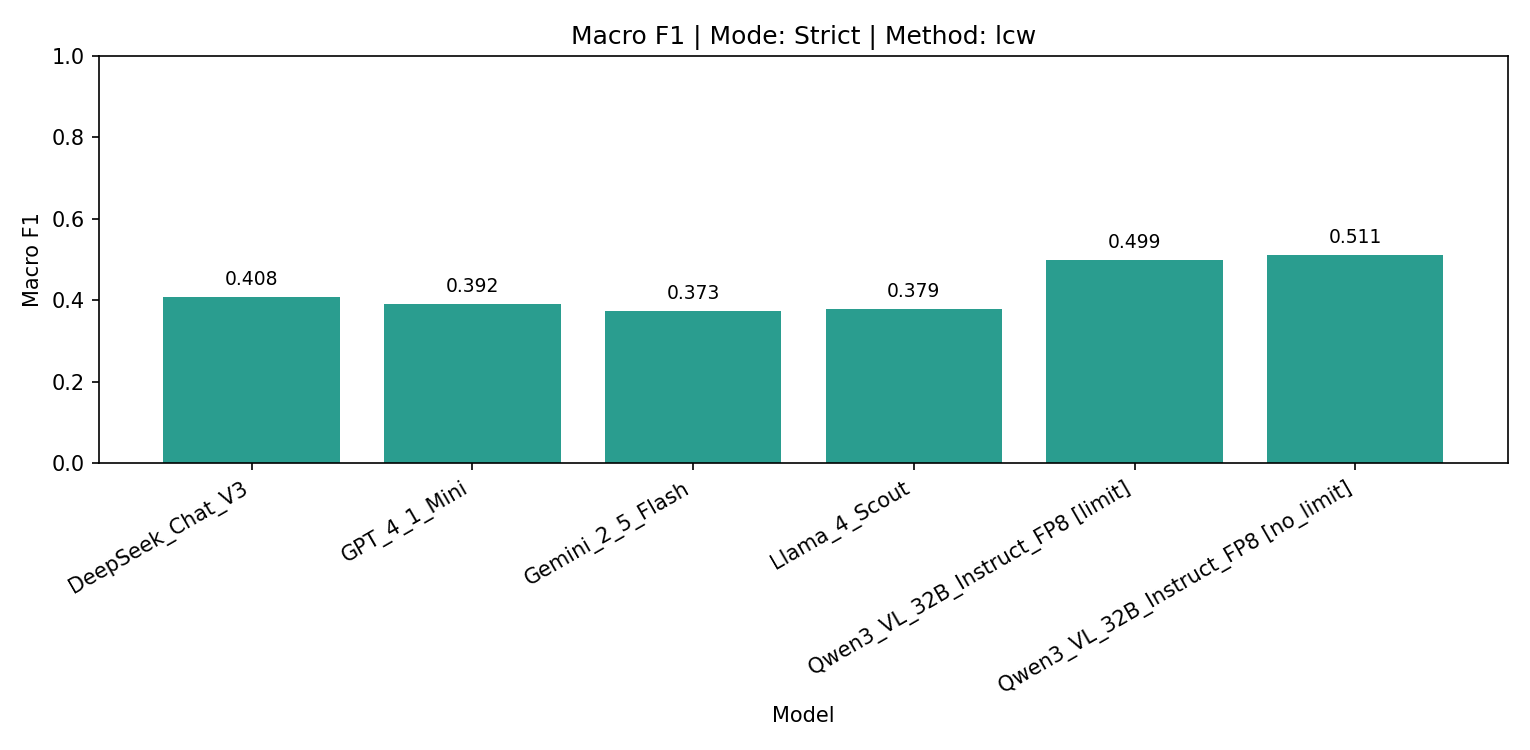
\includegraphics[width=1\textwidth, height=0.6\textheight, keepaspectratio]{figures/results/macro_f1_bar_chart_lcw_strict.png}
    \caption[Bar Chart - Correctness - Macro F1 - LCW]{Comparison of \textit{Macro F1} scores for all models- Method: LCW - Mode: Strict}
    \label{fig:macro_f1_bar_lcw_strict}
\end{figure}
%

\begin{figure}[H]
    \centering
    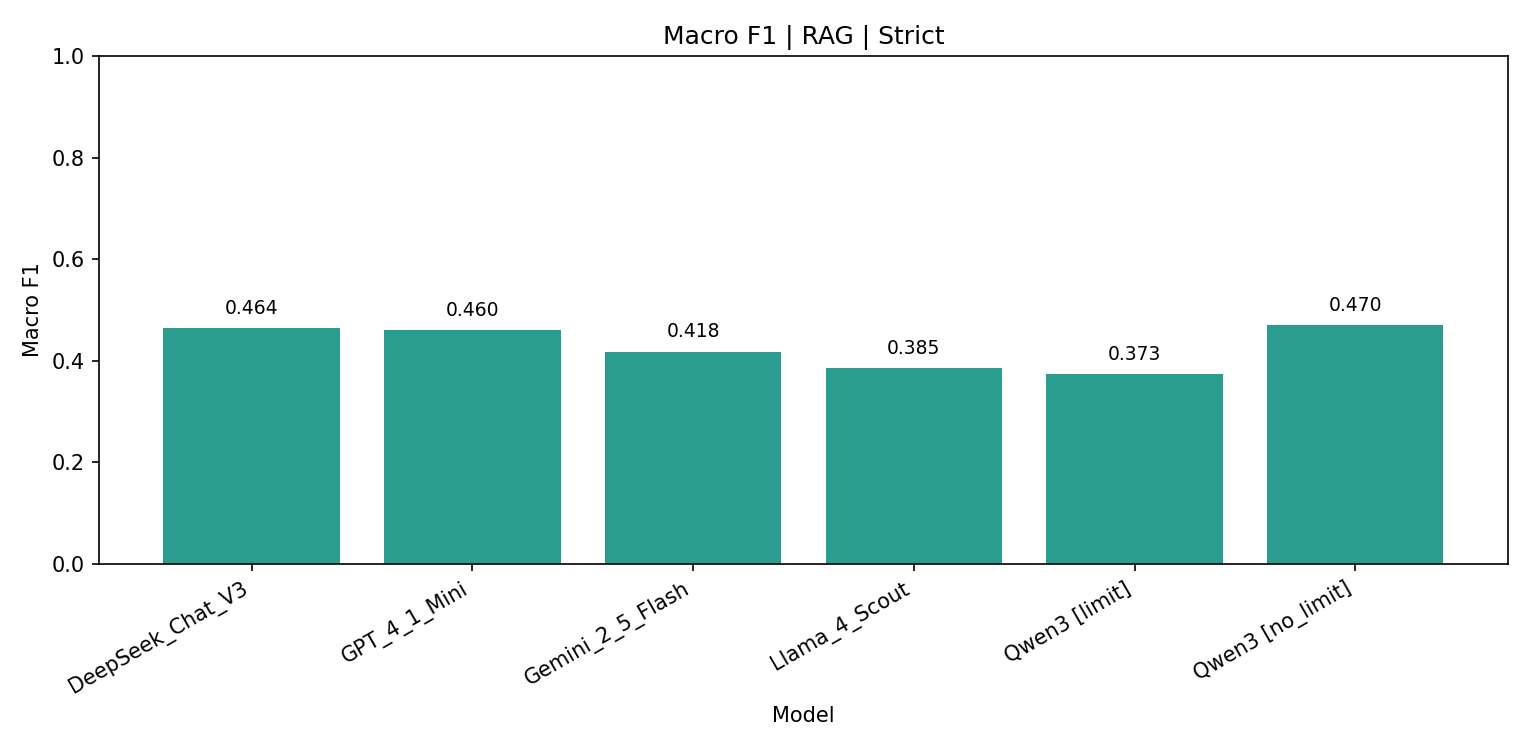
\includegraphics[width=1\textwidth, height=0.6\textheight, keepaspectratio]{figures/results/macro_f1_bar_chart_rag_strict.png}
    \caption[Bar Chart - Correctness - Macro F1 - RAG]{Comparison of \textit{Macro F1} scores for all models- Method: RAG - Mode: Strict}
    \label{fig:macro_f1_bar_rag_strict}
\end{figure}
%

The charts \cref{fig:macro_f1_bar_lcw_strict} and \cref{fig:macro_f1_bar_rag_strict} show a comparison of the Macro \textit{F1} scores between the methods with the underlying point scores assessed in \textit{Strict} mode.

\noindent\textbf{Differences under Strict Mode Evaluation:}
\begin{itemize}
    \item \textbf{Performance Similarities and Differences:} When evaluated in \textit{strict} mode, the \textit{OpenRouter} models show similar results within their respective pipelines.
    In the \ac{lcw} pipeline, the Macro-F1 values are closely clustered between $0.37$ and $0.41$.
    While \textit{DeepSeek-V3} is leading slightly at $0.408$.
    \item \textbf{Performance Difference between Methods:} Switching from \ac{lcw} to \ac{rag} leads to consistent performance improvements a\-cross all \textit{OpenRouter} models.
    This confirms that the targeted retrieval of context prevents the model from being distracted during strict token matching.
    \item \textbf{Comparison between Providers:} In contrast to the \textit{OpenRouter} models, the model \textit{Qwen3-VL-32B} shows the opposite trend. Under \ac{lcw}, \textit{Qwen3-VL-32B} [no\_limit] achieves the highest strict overall score of $0.511$.
    Under \ac{rag}, however, its performance drops to $0.473$ (without limitation) and $0.373$ (with limitation).
\end{itemize}

Overall, the \textit{Qwen3-VL-32B} model outperforms the \textit{OpenRouter} models with an average \textit{F1} score of $0.5$ in large context scenarios.
Specifically, this means that on average the model generates correct subanswers \SI{50}{\%} of the time when answering a question within the \ac{lcw} pipeline. 
At the same time, this implies that, on average, if the model was able to provide all required correct subanswers, it then also provided the same amount of incorrect or irrelevant subanswers.
It is an indicator of knowledge gaps, hallucinations, and deviations from the parsed knowledge base.
However, the results are again to be considered in the context of the evaluation pipeline applied.
%

\begin{figure}[H]
    \centering
    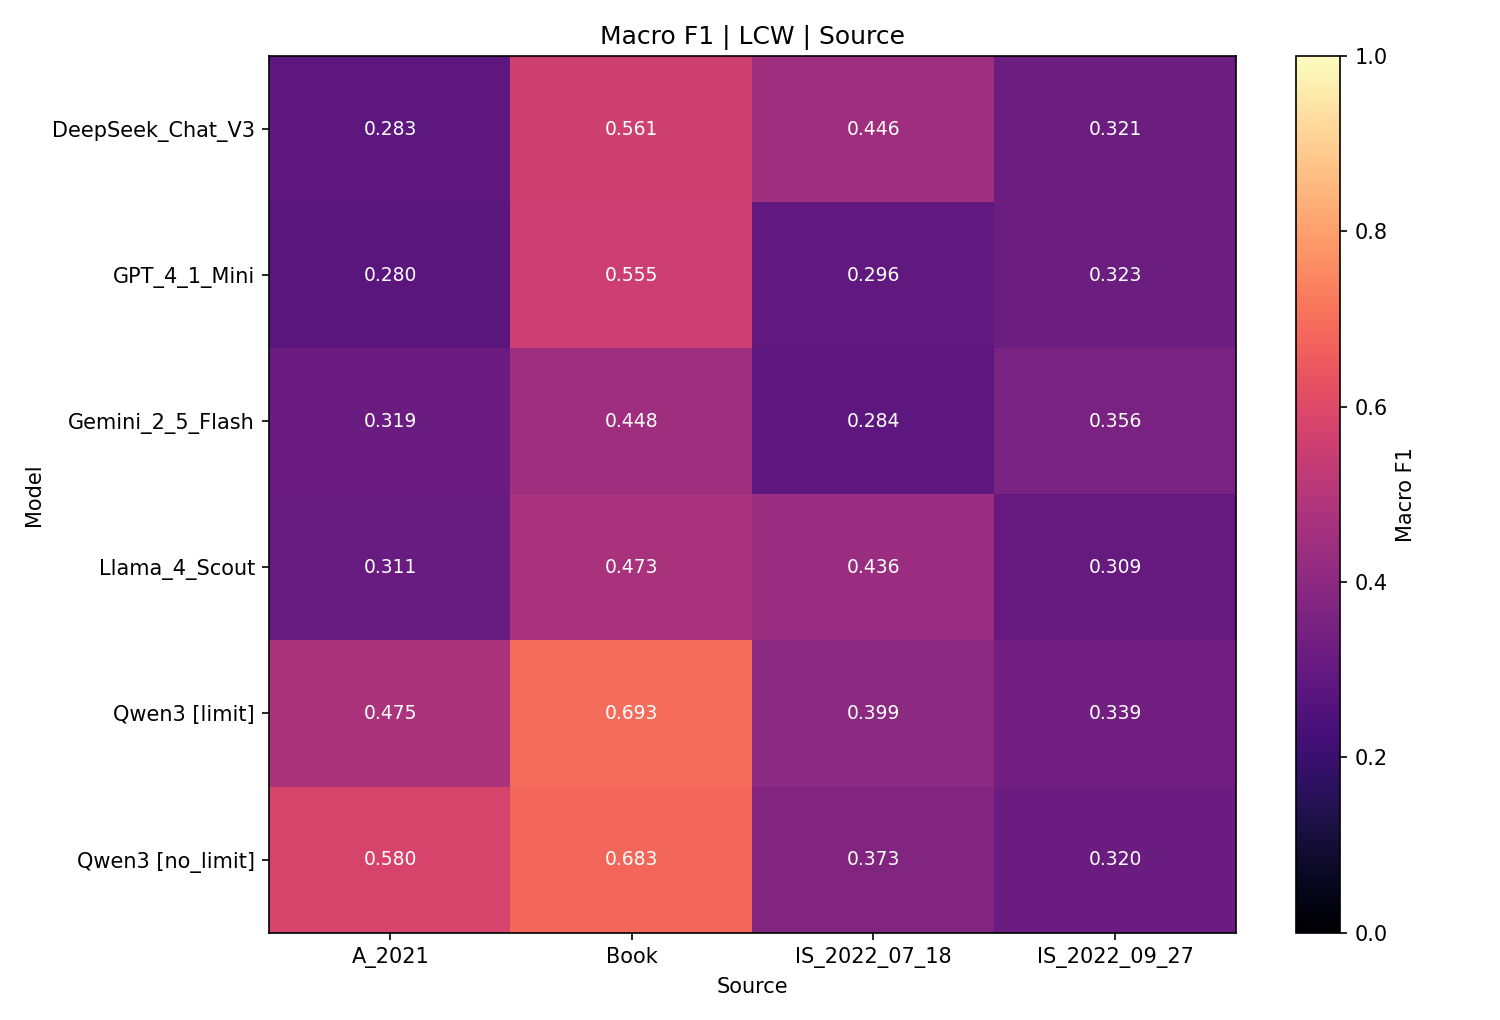
\includegraphics[width=1\textwidth, height=0.5\textheight, keepaspectratio]{figures/results/macro_f1_heatmap_lcw_source_strict.png}
    \caption[Heatmap - Correctness - Macro F1 - LCW]{Heatmap of Macro F1 scores - Method: LCW - Mode: Strict - Grouped by Source}\label{fig:macro_f1_lcw_rag_heat_strict_source}
\end{figure}

\begin{figure}[H]
    \centering
    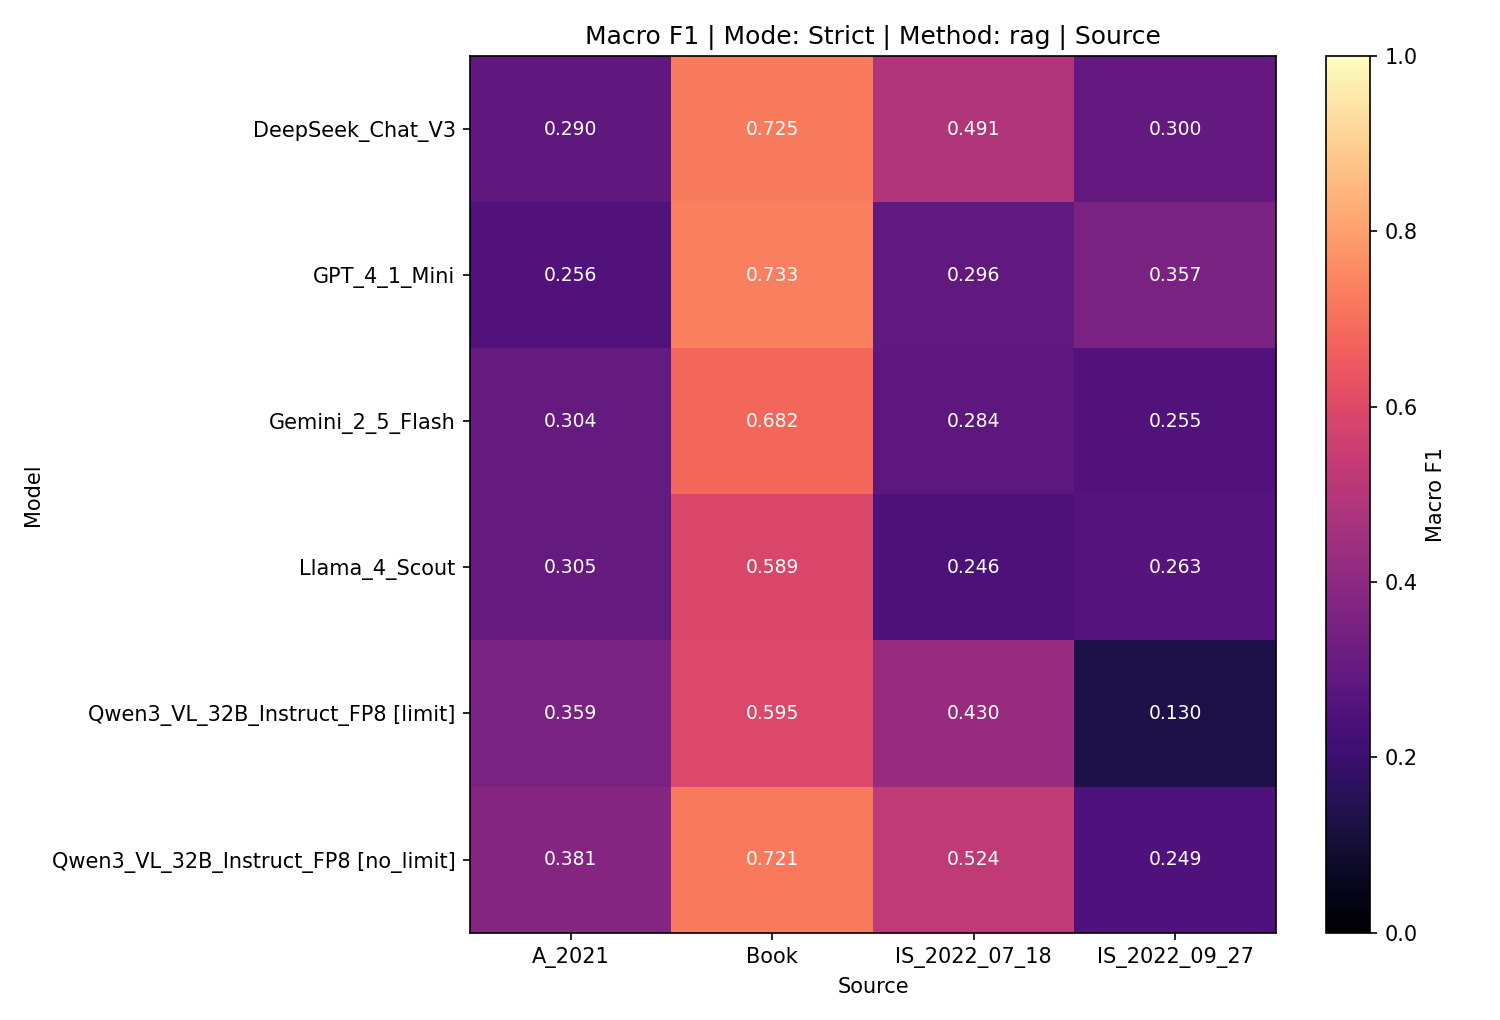
\includegraphics[width=1\textwidth, height=0.5\textheight, keepaspectratio]{figures/results/macro_f1_heatmap_rag_source_strict.png}
    \caption[Heatmap - Correctness - Macro F1 - RAG]{Heatmap of Macro F1 scores - Method: RAG - Mode: Strict - Grouped by Source.}
    \label{fig:macro_f1_rag_strict_heat_exam_source}
\end{figure}

The graphics at \cref{fig:macro_f1_lcw_rag_heat_strict_source} and \cref{fig:macro_f1_rag_strict_heat_exam_source} show the Macro \textit{F1} scores compared by the source of questions.

\noindent\textbf{Key Findings:}
\begin{itemize}
    \item \textbf{Book Questions:} For questions taken directly from the \citetitle{bb2}, there is a clear and significant divergence in performance.
    In the \ac{lcw} pipeline, all \textit{OpenRouter} models achieve very low scores ($F1 \leq 0.15$), with only \textit{Qwen3-VL-32B} [no\_limit] achieving a score of $0.435$.
    In contrast, the scores in the \ac{rag} pipeline increase across the board.
    \textit{DeepSeek-V3} achieves $0.468$ and \textit{GPT-4.1-Mini} $0.518$.
    \item \textbf{Exam collections (A\_2021 \& IS\_2022):} For the exam questions, both pipelines show similar results ranging between $\approx 0.35$ to $0.50$. 
    No clear advantage of either method can be observed.
\end{itemize}
%A more detailed analysis can be found on 
\section{Explainability Analysis}\label{sec:explainability_results}

\begin{figure}[H]
    \centering
    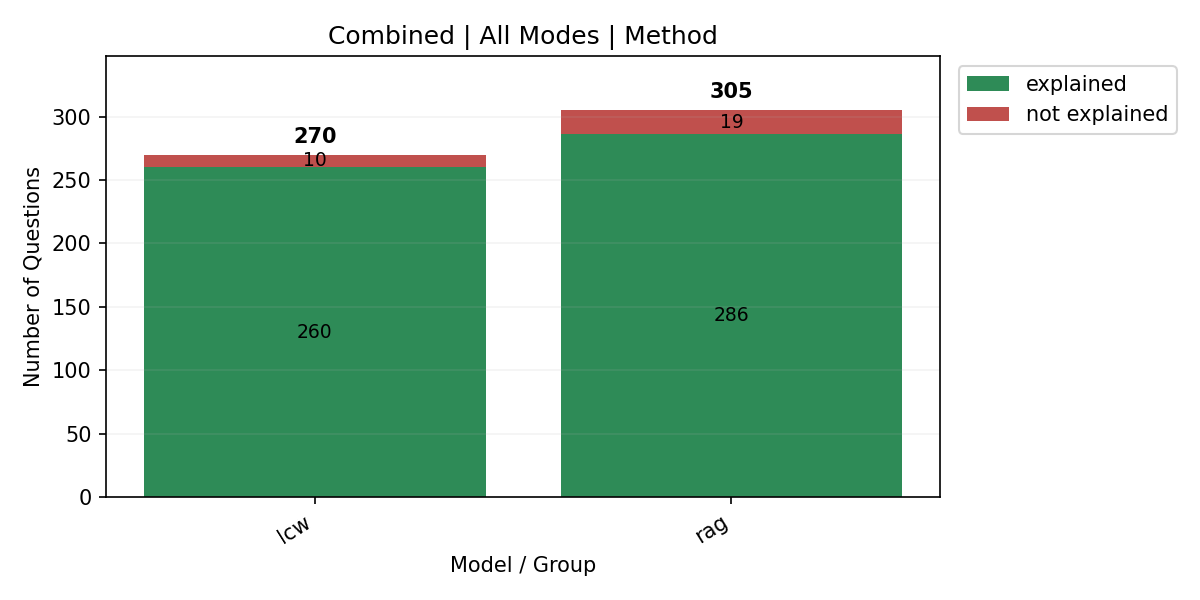
\includegraphics[width=0.9\textwidth, height=0.5\textheight, keepaspectratio]{figures/results/explain_bar_counts_all_models_method.png}
    \caption{Bar chart of Explainability scores for all models combined - Grouped by Method}
    \label{fig:explain_bart_chart_all_models_metho}
\end{figure}

The chart \cref{fig:explain_bart_chart_all_models_metho} shows the total number of questions that were correctly answered, while also containing an explanation, compared by methods. 

The models evaluated within the method pipelines demonstrate a high ability to provide explanations within the generated answer.
This result is particularly notable, as the prompt used does not explicitly require the model to provide an explanation.

Only questions that were previously evaluated as correctly answered were taken into account.
The significant percentage of correctly answered questions without an explicit explanation is most likely due to the character of the question.

For example, if the question asks for a comparison of two hospital information systems in tabular form, the respective \ac{lm} adheres to the requested format, which subsequently leaves little room for an explanation.
%
\section{Question Understanding Analysis}\label{sec:question_understanding}
The number of answers generated and evaluated as \enquote{understood} is not equivalent to the number of answers evaluated by the \textit{Correctness} metric.
A question is not automatically considered as \enquote{understood} if it has been answered.
Certain questions may have been answered; however, the answers contain incorrect facts or information unrelated to the initial question.
These answers are counted as \enquote{not understood}.
At the same time, an answer evaluated as \enquote{not answered} in relation to the question can be counted as \enquote{understood}.
In some cases, a \ac{lm} generated an answer that explains why the model could not answer the question.
The resulting answer does not provide useful information or knowledge, but clearly shows an understanding of the question.
%

\begin{figure}[htbp]
    \centering
    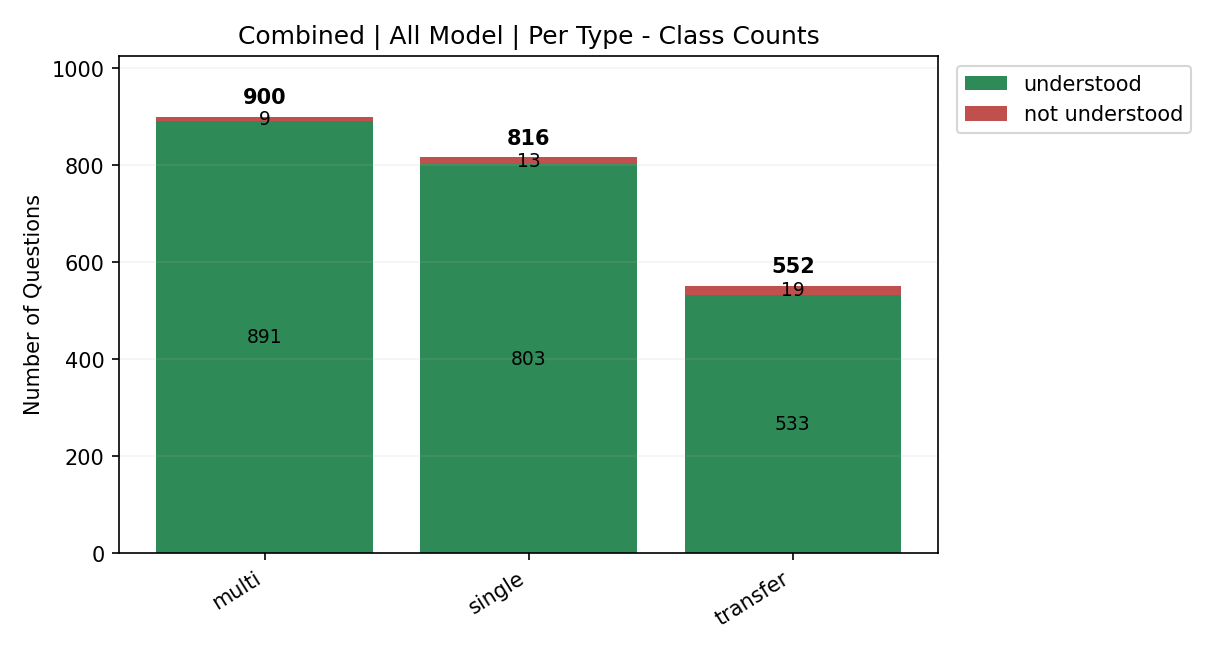
\includegraphics[width=0.9\textwidth, height=0.4\textheight, keepaspectratio]{figures/results/understandability_total_per_type.png}
    \caption[Bar chart - Understandibility]{Bart Chart - Understandability - Total - Grouped by Type.}
    \label{fig:understandability_total_type}
\end{figure}
%

\cref{fig:understandability_total_type} shows the total number of questions \enquote{understood} by the models evaluated in relation to those \enquote{not understood}.
%
In contrast to the \textit{Explainability} criterion, all existing questions were assessed for \textit{Question Understanding}.
All models show high success rates within both methods.
However, a few more questions of type \textit{transfer} were not understood.
Similarly to the previous metrics, the questions assessed as \textit{not understood} are not a representation of the performance of the \ac{lm} or method.

Within the pipelines, a misunderstanding is mainly caused by a prior \ac{api} error or a nonsense output that was repeatedly reproduced.
Such cases should therefore not be included in the overall assessment and would result in an even better score for all models.
%
\section{Robustness Analysis}

In order to assess the \textit{Robustness} of the models and methods, all question sets were duplicated and inserted with spelling errors.
The subsequently generated answers were also evaluated using the \textit{F1} metric. 

The introduction of spelling errors could result in different \textit{chunks} being retrieved from the \ac{db}.
For the \ac{rag} method, it is essentially a test of the robustness of the similarity search.
How flexible is the retrieval system?

For the \ac{lcw} method, it is the problem of the \enquote{needle in the haystack}.
At this point, this raises the particular question:\\
Is the required \enquote{reproduction} of knowledge during inference and generation robust when the inputs are ambiguous or inconsistent?

\acp{lm} are trained on \enquote{natural language}, which therefore regularly contains spelling errors.
It is therefore to be expected that the quality of output remains rather stable.

%
%LCW-Robustness
\begin{figure}[htbp]
    \centering
    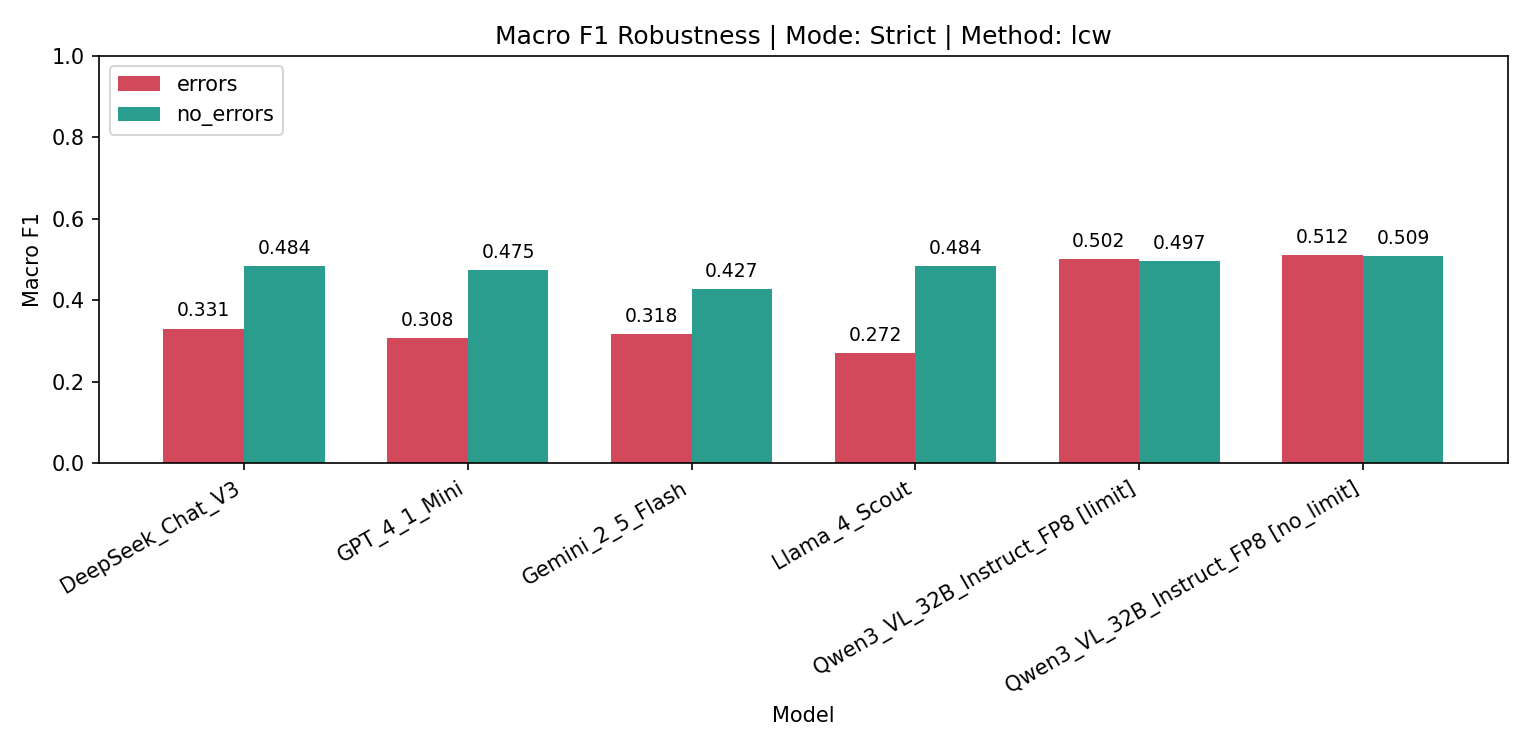
\includegraphics[width=0.95\textwidth, height=0.5\textheight, keepaspectratio]{figures/results/macro_f1_robustness_bar_chart_strict_lcw.png}
    \caption[Robustness - Macro F1 - LCW]{Robustness - Comparison of Macro F1 scores by question error/spelling status - Method: LCW}
    \label{fig:robustness_f1_lcw}
\end{figure}
%

The chart \cref{fig:robustness_f1_lcw} shows a comparison of the Macro \textit{F1} scores by the error status of the input question during inference within the \ac{lcw} method.

%RAG - Robustness
\begin{figure}[htbp]
    \centering
    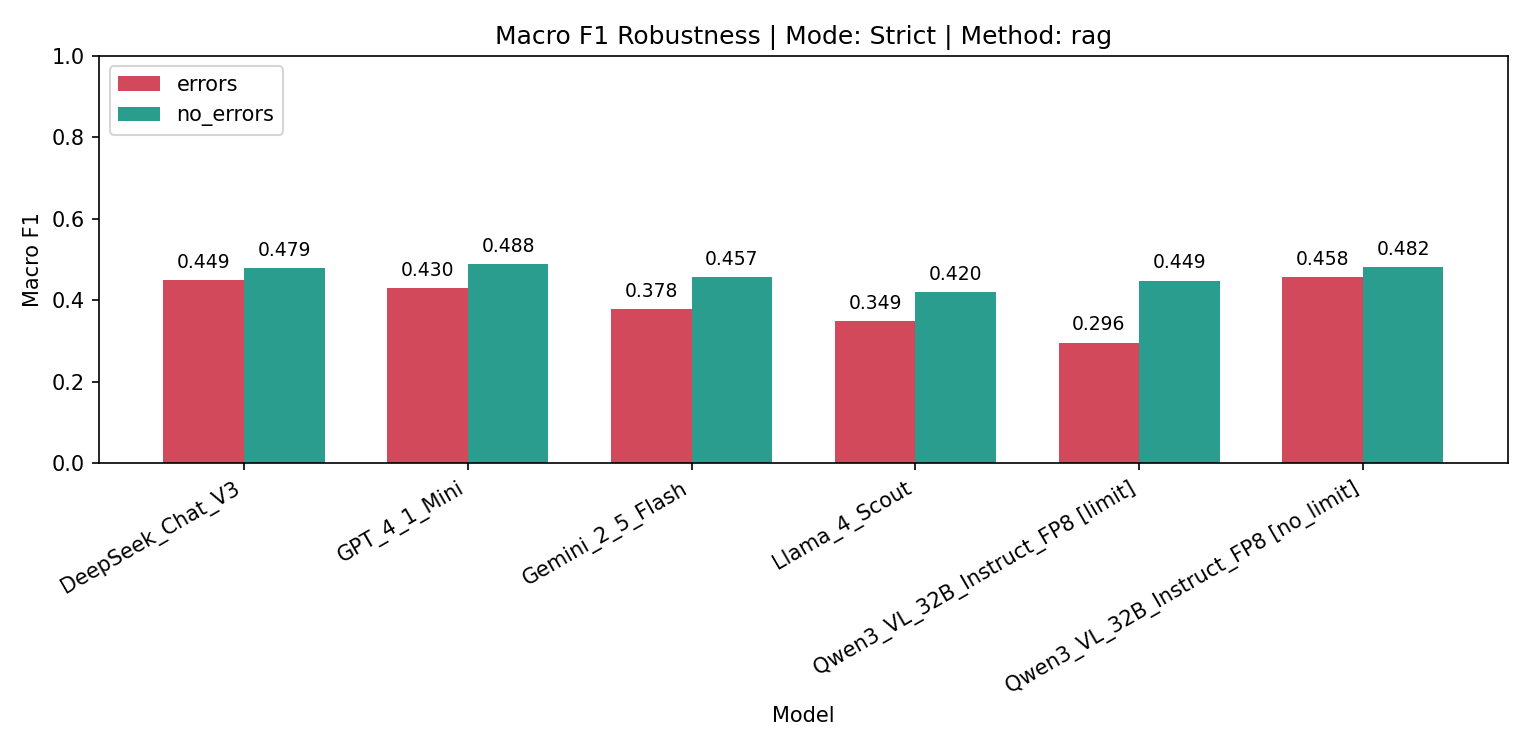
\includegraphics[width=0.95\textwidth, height=0.5\textheight, keepaspectratio]{figures/results/macro_f1_robustness_bar_chart_strict_rag.png}
    \caption[Robustness - Macro F1 - RAG]{Robustness - Comparison of Macro F1 scores by question error status - Method: RAG}
    \label{fig:robustness_f1_rag}
\end{figure}
%

The chart \cref{fig:robustness_f1_rag} shows a comparison of the Macro \textit{F1} scores by the error status of the input question during inference within the \ac{rag} method.

The results presented in \cref{fig:robustness_f1_lcw} and \cref{fig:robustness_f1_rag} partially confirm the assumptions made earlier.

For the \ac{lcw} method (\cref{fig:robustness_f1_lcw}), the results clearly demonstrate that the inserted spelling errors lead to a decrease in output quality.
It is noteworthy, however, that this decline is only evident in the \textit{OpenRouter} models.
For the \textit{Llama} model, the values differ by \SI{21}{\%}, which makes the model almost unusable in a real-world application within the setup used in this work.
It should be noted that the values must always be considered within the context of the methodological framework presented.

The \textit{Qwen3} model counterintuitively shows a small increase in the respective scores.

For the \ac{rag} method (\cref{fig:robustness_f1_rag}), the Macro \textit{F1} results suggest that inserted spelling errors do have a negative impact on the retrieval process.

The Macro \textit{F1} scores are consistently lower for the processed questions.
The most significant difference is present for the \textit{Qwen3} [limit] results, where the score drops by $15$ percentage points.  
For the other models, the score decreases between \SI{2}{\%} and \SI{7}{\%}.
Among other things, this result shows that the application requires preprocessing in a real-world scenario.

The probability that users will formulate every query without errors is very low and clearly leads to a loss of quality.
Preprocessing of user input would be needed to correct such factors.

\section{Summary}

In general, it is not possible to make a definitive statement about which method is generally the better choice.
As stated earlier in \cref{res:key_findings}, the respective values vary between the models, showing a slight superiority of \ac{rag} with no consistent pattern.

For the \textit{OpenRouter} models, the \ac{rag} method demonstrates superior performance based on the \textit{F1} scores.

For the \textit{Qwen} model, the performance is the opposite of that seen in the \textit{OpenRouter} models. 
Here, the \ac{lcw} method produces better and more robust results.

All models show a high to perfect level of \textit{Understandability} and \textit{Explainability}.
The corresponding scores are not surprising, but rather reflect the current state of development of \acp{llm}.

The assessment of \textit{Correctness} yields sobering results but, as already mentioned, must be viewed within the context of the methodological framework.

The nuances involved in evaluating answers in a domain that is based on hard, unambiguous facts cannot, or can only with great difficulty, be fully defined in a prompt.
The \textit{Exam} mode and the combination of correct and partially correct answers attempted to approach the evaluation process with a broader perspective.
The resulting assessment might be valuable to the user group and future work.

The evaluation process can be extended and refined.
